
\chapter{Instrumentation cyber-security}

As digital technology finds greater application in industrial measurement and control systems, these systems become subject to digital vulnerabilities.  Cyber-security, which used to be strictly limited to information technology (IT) systems such as those used in office and research environments (e.g. desktop computers, printers, internet routers), is now a pressing concern for industrial measurement and control systems.  \index{Information Technology (IT)}

There exist many points of commonality between digital IT and digital control systems, and it is at these points where mature protection concepts may be borrowed from the world of IT for use protecting industrial control systems.  However, digital measurement and control systems have many unique features, and it is here we must develop protection strategies crafted specifically for industrial applications.

The chief difference between industrial controls and IT systems is, of course, the fact that industrial controls directly manage real physical processes.  The purpose of an IT system, in contrast, is to manage \textit{information}.  While information can be dangerous in the wrong hands, physical processes such as chemical plants, nuclear power stations, water treatment facilities, hazardous waste treatment facilities, can be even more so.

This chapter will primarily focus on digital security as it applies to industrial measurement and control systems.  The opening section is a case study on what has become a famous example of an industrial-scale cyber-attack: the so-called \textit{Stuxnet} virus.

\vskip 10pt

As control system professionals, it is in our interest to ensure our measurement and control systems are secure from unauthorized access.  It is helpful to regard system \textit{security} similarly to how we regard system \textit{safety} or \textit{reliability}, as these concerns share many common properties:

\begin{itemize}
\item Just as accidents and faults are inevitable, so is unauthorized access to any digital system
\item Just as 100\% perfect safety and 100\% perfect reliability is unattainable, so is 100\% security
\item Digital security needs to be an important criterion in the selection and setup of industrial instrumentation equipment, just as safety and reliability are important criteria
\item Maximizing security requires a security-savvy culture within the organization, just as maximizing safety requires a safety-savvy culture and maximizing reliability requires a reliability-centric design philosophy
\end{itemize}

Also similar to safety and reliability is the philosophy of \textit{defense-in-depth}, which is simply the idea of having multiple layers of protection in case one or more fail.  Applied to digital security, defense-in-depth means not relying on a single mode of protection (e.g. passwords only) to protect a system from attack.  \index{Defense-in-depth}  \index{Passwords}


%Above all, one must avoid falling prey to the assumption that ``this couldn't happen to me''.  The attitude we should carry, by contrast, is one that recognizes \textit{any} system can be compromised.


\vskip 10pt

It should be noted that cyber-security is a very complex topic, and that this chapter of the book is quite unfinished at the time of this writing (2016).  Later versions of the book will likely have much more information on this important topic.








\filbreak
\section{Stuxnet}

In November of 2007 a new computer virus was submitted to a virus scanning service.  The purpose of this new virus was not understood at the time, but it was later determined to be an early version of the so-called \textit{Stuxnet} virus which was designed to infiltrate and attack programmable logic controllers (PLCs) installed at the uranium enrichment facility in Iran, a critical part of that country's nuclear program located in the city of Natanz.  Stuxnet stands as the world's first known computer virus ever designed to specifically attack an industrial control platform, in this case Siemens model S7 PLCs.  \index{Stuxnet computer virus}

Later forensic analysis revealed the complexity and scope of Stuxnet for what it was: a digital weapon, directed against the Iranian nuclear program for the purpose of delaying that program's production of enriched uranium.  Although the origins of Stuxnet are rather unique as viruses go, the lessons learned from Stuxnet help us as industrial control professionals to fortify our own control systems against similarly-styled digital attacks.  The next such attack may not come from a nation-state like Stuxnet did, but you can be sure whoever attacks next will have gained from the lessons Stuxnet taught the world.

Since the Stuxnet attack was directed against a nuclear facility, it is worthwhile to know a little about what that facility did and how it functioned.  The next subsection will delve into some of the details of modern uranium enrichment processes, while further subsections will outline how Stuxnet attacked those physical processes through the PLC control system.

The sections following this one on Stuxnet will broaden the scope of the conversation to vulnerabilities and fortifications common to many industrial control networks and systems.






\filbreak
\subsection{A primer on uranium enrichment}

Uranium is a naturally occurring metal with interesting properties lending themselves to applications of nuclear power and nuclear weaponry.  Uranium is extremely dense, and also (mildly) radioactive.  Of greater importance, though, is that some of the naturally occurring isotopes\footnote{The term \textit{isotope} refers to differences in atomic mass for any chemical element.  For example, the most common isotope of the element \textit{carbon} (C) has six neutrons and six protons within each carbon atom nucleus, giving that isotope an atomic mass of twelve ($^{12}$C).  A carbon atom having two more neutrons in its nucleus would be an example of the isotope $^{14}$C, which just happens to be radioactive: the nucleus is unstable, and will over time \textit{decay}, emitting energy and particles and in the process change into another element.} of uranium are \textit{fissile}, which means those atoms may be easily ``split'' by neutron particle bombardment, releasing huge amounts of energy as well as more neutrons which may then go on to split more uranium atoms in what is called a \textit{chain reaction}.  Such a chain-reaction, when controlled, constitutes the energy source of a fission reactor.  Nuclear weapons employ violently uncontrolled chain reactions.  \index{Fission, nuclear}  \index{Chain reaction, nuclear}  \index{Isotope}

The most fissile isotope of uranium is uranium 235, that number being the total count of protons and neutrons within the nucleus of each atom.  Unfortunately (or fortunately, depending on your view of nuclear fission), $^{235}$U constitutes only 0.7\% of all uranium found in the earth's crust.  The vast majority of naturally occurring uranium is the isotope $^{238}$U which has all the same chemical properties of $^{235}$U but is non-fissile (i.e. an atom of $^{238}$U will not be ``split'' by neutron particle bombardment\footnote{It is noteworthy that $^{238}$U can be converted into a different, fissile element called plutonium through the process of neutron bombardment.  Likewise, naturally-occurring thorium 232 ($^{232}$Th) may be converted into $^{233}$U which is fissile.  However, converting non-fissile uranium into fissile plutonium, or converting non-fissile thorium into fissile uranium, requires intense neutron bombardment at a scale only seen within the core of a nuclear reactor running on some other fuel such as $^{235}$U, which makes $^{235}$U the critical ingredient for any independent nuclear program.}).

Naturally-occurring uranium at a concentration of only 0.7\% $^{235}$U is too ``dilute'' for most\footnote{Power reactors using ``heavy'' water as the moderator (such as the Canadian ``CANDU'' design) are in fact able to use uranium at natural $^{235}$U concentration levels as fuel, but most of the power reactors in the world do not employ this design.} nuclear reactors to use as fuel, and certainly is not concentrated enough to construct a nuclear weapon.  Most power reactors require uranium fuel at a $^{235}$U concentration of at least 3\% for practical operation, and a concentration of at least 20\% is considered the low threshold for use in constructing a uranium-based nuclear weapon.  Mildly concentrated uranium useful for reactor fuel is commonly referred to ``low-enriched uranium'' or \textit{LEU}, while uranium concentrated enough to build a nuclear weapon is referred to as ``highly enriched uranium'' or \textit{HEU}.  Modern uranium-based nuclear bombs rely on the uranium being concentrated to at least 90\% $^{235}$U, as do military power reactors such as the extremely compact designs used to power nuclear submarines.  All of this means that an industrial-scale process for concentrating (enriching) $^{235}$U is a necessary condition for building and sustaining a nuclear program of any kind, whether its purpose be civilian (power generation, research) or military (weapons, nuclear-powered vehicles).  \index{CANDU nuclear reactor}  \index{LEU}  \index{HEU}  \index{Enriched uranium}

Different technologies currently exist for uranium enrichment, and more are being developed.  The technical details of uranium enrichment set the background for the Stuxnet story, the site of this cyber-attack being the Natanz uranium enrichment facility located in the middle-eastern nation of Iran.

\vskip 10pt

\filbreak

Like all 2-phase separation processes, uranium enrichment breaks a single input ``feed'' stream into two out-going streams of differing composition.  Since in the case of uranium enrichment only one stream is of strategic interest, the stream containing concentrated $^{235}$U is called the \textit{product}.  The other stream coming exiting the separation process, having been largely depleted of valuable $^{235}$U, is called the \textit{tails}:

$$\includegraphics{security_03.eps}$$

During the United States' Manhattan Project of World War Two, the main process chosen to enrich uranium for the first atomic weapons and industrial-scale reactors was \textit{gaseous diffusion}.  In this process, the uranium metal is first chemically converted into \textit{uranium hexafluoride} (UF$_{6}$) gas so that it may be compressed, transported through pipes, processed in vessels, and controlled with valves.  Then, the UF$_{6}$ gas is run through a long series of diffusion membranes (similar to fine-pore filters).  At each membrane, those UF$_{6}$ molecules containing $^{235}$U atoms will preferentially cross through the membranes because they are slightly less massive than the UF$_{6}$ molecules containing $^{238}$U atoms.  The mass difference between the two isotopes of uranium is so slight, though, that this membrane diffusion process must be repeated thousands of time in order to achieve any significant degree of enrichment.  Gaseous diffusion is therefore an extremely inefficient process, but nevertheless one which may be scaled up to industrial size and used to enrich uranium at a pace sufficient for a military nuclear program.  At the time of its construction, the world's first gaseous diffusion enrichment plant (built in Oak Ridge, Tennessee) also happened to be the world's largest industrial building.

An alternative uranium enrichment technology considered but later abandoned by the Manhattan Project scientists was \textit{gas centrifuge} separation.  A gas centrifuge is a machine with a hollow rotor spun at extremely high speed.  Gas is introduced into the interior of the rotor, where centrifugal force causes the heavier molecules to migrate toward the walls of the rotor while keeping the lighter molecules toward the center.  Centrifuges are commonly used for separating a variety of different liquids and solids dissolved in liquid (e.g. separating cells from plasma in blood, separating water from cream in milk), but gas centrifuges face a much more challenging task because the difference in density between various gas molecules is typically far less than the density differential in most liquid mixtures.  This is especially true when the gas in question is uranium hexafluoride (UF$_{6}$), and the only difference in mass between the UF$_{6}$ molecules is that caused by the miniscule\footnote{The formula weight for UF$_{6}$ containing fissile $^{235}$U is 349 grams per mole, while the formula weight for UF$_{6}$ containing non-fissile $^{238}$U is only slightly higher: 352 grams per mole.  Thus, the difference in mass between the two molecules is less than one percent.} difference in mass between the uranium isotopes $^{235}$U and $^{238}$U.  \index{Centrifuge}  \index{Gas centrifuge}

\vskip 10pt

\filbreak

Gas centrifuge development was continued in Germany, and then later within the Soviet Union.  The head of the Soviet gas centrifuge effort -- a captured Austrian scientist named Gernot Zippe -- was eventually brought to the United States where he shared the refined centrifuge design with American scientists and engineers.  As complex as this technology is, it is far\footnote{By some estimates, gas centrifuge enrichment is 40 to 50 \textit{times} more energy efficient than gaseous diffusion enrichment.} more energy-efficient than gas diffusion, making it the uranium enrichment technology of choice at the time of this writing (2016).

An illustration of Gernot Zippe's design is shown below.  The unenriched UF$_{6}$ feed gas is introduced into the middle of the spinning rotor where it circulates in ``counter-current'' fashion both directions parallel to the rotor's axis.  Lighter ($^{235}$U) gas tends to stay near the center of the rotor and is collected at the bottom by a stationary ``scoop'' tube where the inner gas current turns outward.  Heavier ($^{238}$U) gas tends to stay near the rotor wall and is collected at the top by another stationary ``scoop'' where the outer current turns inward:

$$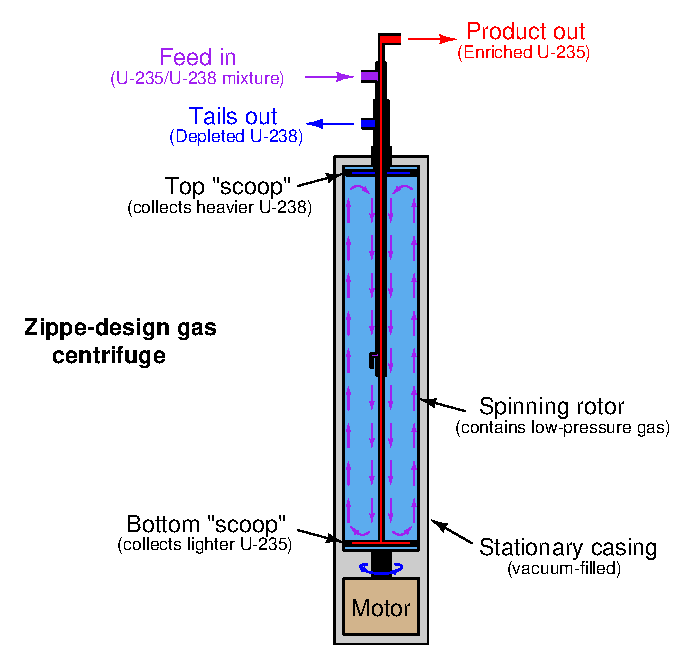
\includegraphics{security_01.eps}$$

\vskip 10pt

Like the separation membranes used in gaseous diffusion processes, each gas centrifuge is only able to enrich the UF$^{6}$ gas by a very slight amount.  The modest enrichment factor of each centrifuge necessitates many be connected in series, with each successive centrifuge taking in the out-flow of the previous centrifuge in order to achieve any practical degree of enrichment.  Furthermore, gas centrifuges are by their very nature rather limited in their flow capacity\footnote{A typical gas centrifuge's mass flow rating is on the order of milligrams per second.  At their very low (vacuum) operating pressures, a typical centrifuge rotor will hold only a few grams of gas at any moment in time.}.  This low ``throughput'' necessitates parallel-connected gas centrifuges in order to achieve practical production rates for a national-scale nuclear program.  A set of centrifuges connected in parallel for higher flow rates is called a \textit{stage}, while a set of centrifuge stages connected in series for greater enrichment levels is called a \textit{cascade}.  \index{Gas centrifuge stage}  \index{Gas centrifuge cascade}

A gas centrifuge \textit{stage} is very simple to understand, as each centrifuge's feed, product, and tails lines are simply paralleled for additional throughput:

$$\includegraphics{security_04.eps}$$

A gas centrifuge \textit{cascade} is a bit more complex to grasp, as each centrifuge's product gets sent to the feed inlet of the next stage for further enrichment, and the tails gets sent to the feed inlet of the previous stage for further depletion.  The main feed line enters the cascade at one of the middle stages, with the main product line located at one far end and the main tails line located at the other far end:

$$\includegraphics{security_05.eps}$$

\vskip 10pt

\filbreak

This US Department of Energy (DOE) photograph shows an array of 1980's-era American gas centrifuges located in Piketon, Ohio.  Each of the tall cylinders is a single gas centrifuge machine, with the feed, product and tails tubing seen connecting to the spinning rotor at the top of the stationary casing:

$$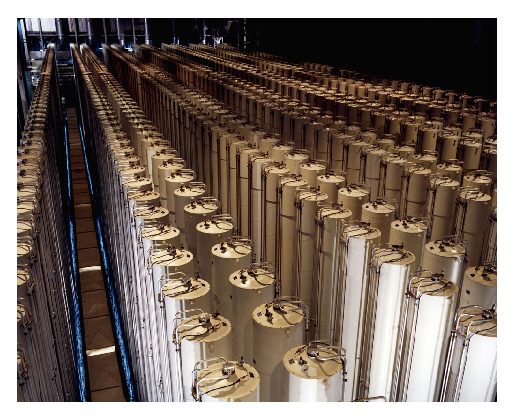
\includegraphics[width=6in]{security_02.eps}$$

\vskip 10pt

\filbreak

The size of each stage in a gas centrifuge cascade is proportional to its feed flow rate.  The stage processing the highest feed rate must be the largest (i.e. contain the most centrifuges), while the stages at the far ends of the cascade contain the least centrifuges.  A cascade similar to the one at the Natanz enrichment facility in Iran -- the target of the Stuxnet cyber-attack -- is shown here without piping for simplicity, consisting of 164 individual gas centrifuges arranged in 15 stages.  The main feed enters in the middle of the cascade at the largest stage, while enriched product exits at the right-hand end and depleted tails at the left-hand end:

$$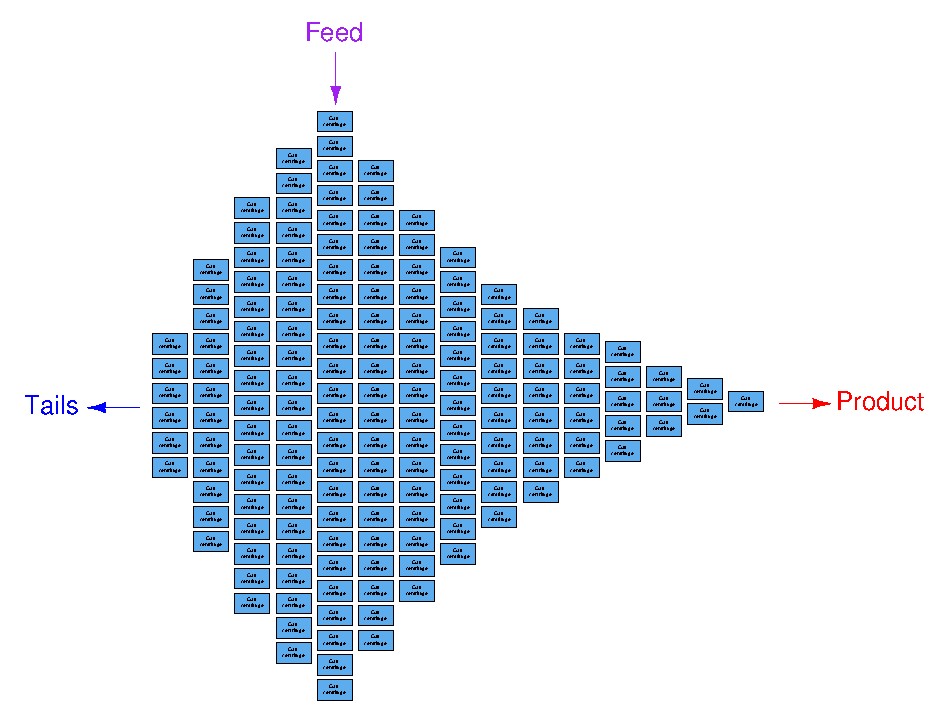
\includegraphics{security_06.eps}$$

The sheer number of gas centrifuges employed at a large-scale uranium enrichment facility is quite staggering.  At the Natanz facility, where just one cascade contained 164 centrifuges, cascades were paralleled together in \textit{sub-units} of six cascades each (984 centrifuges per sub-unit), and three of these sub-units made one cascade \textit{unit} (2952 centrifuges total).






\filbreak
\subsection{Gas centrifuge vulnerabilities}

It would be an understatement to say that a gas centrifuge is a delicate machine.  In order to perform their task efficiently\footnote{Three major factors influence the efficiency of a gas centrifuge: rotor wall speed, rotor length, and gas temperature.  Of these, rotor wall speed is the most influential.  Higher speeds separate isotopes more effectively, because higher wall speeds result in greater amounts of radial acceleration, which increases the amount of centrifugal force experienced by the gas molecules.  Longer rotors also separate isotopes more effectively because they provide more opportunity for the counter-flowing gas streams to separate lighter molecules toward the center and heavier molecules toward the wall.  Higher temperatures reduce separation efficiency, because gas molecules at higher temperatures are more mobile and therefore diffuse (i.e. mix together) at higher rates.  Therefore, the optimum gas centrifuge design will be long, spin as fast as possible, and operate as cool as possible.}, gas centrifuge rotors must be long and made to rotate at extremely high rates of speed.  Maintaining any rotating machine in a state of near-perfect balance is difficult, much more so when the rotating element is very long\footnote{To give you an idea of just how long some gas centrifuge rotors are, the units built for the US Department of Energy facility in Ohio used rotors \textit{40 feet in length}!}.  Furthermore, since the gas pressure inside each centrifuge rotor is sub-atmospheric, leak-free seals must be maintained between the spinning rotor and the stationary components (the casing and internal tubing).  The extremely high rotational speeds of modern gas centrifuges (many tens of thousands of revolutions per minute!) necessitate advanced materials be used in rotor construction, optimizing light weight and high strength so that the rotors will not be torn to pieces by their own centrifugal force.

\vskip 10pt

A peculiar problem faced by any high-speed rotating machine is a phenomenon called \textit{critical speed}.  Any object possessing both mass and resilience is capable of oscillating, which of course includes any and every rotating machine component.  If the rotating component of a machine happens to spin at a rate equal to its own natural oscillating frequency, a condition of \textit{mechanical resonance} occurs.  \textit{Any} amount of imbalance in the rotating component while spinning at this speed, however slight, will generate a force driving the assembly into continuous oscillation.  The speed at which this resonance occurs is called the ``critical speed'' of the machine, and it should be avoided whenever possible.  \index{Critical speed, rotating machine}   \index{Resonance, mechanical}

Destructive resonance will be avoided so long as the machine is maintained at any speed significantly below or above its critical speed.  Most modern gas centrifuges are classified as \textit{supercritical} machines, because they are designed to operate at rotational speeds exceeding their critical speeds.  The only time resonance becomes a problem in a supercritical machine is during start-up and shut-down, when the speed must momentarily pass through the critical value.  So long as this moment is brief, however, oscillations will not have enough time to grow to destructive levels.

\vskip 10pt

In addition to the problems faced by all high-speed rotating machines, a problem unique to gas centrifuges is gas pressure control.  Since the rotor of a gas centrifuge spins inside of an evacuated\footnote{This means the hollow casing exists in a state of vacuum, with no air or other gases present.  This is done in order to help thermally insulate the rotor from ambient conditions, as well as avoid generating heat from air friction against the rotor's outside surface.  Remember, elevated temperatures cause the gas to diffuse at a faster rate, which in turn causes the gas to randomly mix and therefore not separate into light and heavy isotopes as intended.} stationary casing, the existence of any gas pressure inside the rotor creates additional stress acting in the same outward direction as the rotor's own centrifugal force.  This means rotor gas pressure must be maintained at a very low level in order to minimize rotor stress.  Furthermore, if pressure and temperature conditions are not carefully controlled in a gas centrifuge, the gas may actually \textit{sublimate} into a solid state which will deposit material on the inside wall of the rotor and surely throw it out of balance.  \index{Sublimation, phase change}

\vskip 10pt

One could argue that the temperamental nature of gas centrifuges is a good thing, because it makes the manufacture of enriched uranium difficult to achieve, which in turn complicates the development of nuclear weapons.  This fragility also makes gas centrifuges an ideal target for anyone interested in halting or delaying nuclear weapons development, which was precisely the aim of the Stuxnet computer virus.






\filbreak
\subsection{The Natanz uranium enrichment facility}

Iran used an obsolete gas centrifuge design, perhaps the best they could obtain at the time, as the uranium enrichment platform of choice for their Natanz facility.  By modern standards, this design was inefficient and troublesome, but the Iranians were able to coax serviceable performance from this centrifuge design by means of extensive instrumentation and controls.  

Simply put, the Iranian strategy was to manufacture centrifuges faster than they would break and equip the centrifuge cascades with enough piping and supervisory instrumentation that they could detect and isolate failed centrifuges without stopping production, rather than wait until they had perfected the design of the centrifuges themselves.  The extensive network of sensors, valves, piping, and PLCs (Programmable Logic Controllers) installed at the Natanz facility facilitated this fault-tolerant design.

\vskip 10pt

The key to the Natanz system's fault tolerance was a set of isolation (``block'') valves installed at each gas centrifuge.  Each machine was also equipped with a sufficient array of sensors to detect malfunctions.  If a centrifuge experienced trouble, such as excessive vibration, the PLC control system would automatically shut all the isolation valves for that failed centrifuge and turn off its drive motor.  Since most stages in each cascade contained multiple centrifuges in parallel, the isolation of a single centrifuge within a stage would not shut down the entire cascade.  Instead, maintenance personnel could repair the failed centrifuge while production continued, and return it to service when ready.

One undesired consequence of shutting isolation valves on operating centrifuges, though, was increased gas pressure in portions of the cascade.  With fewer centrifuges left to handle a constant feed flow, the pressure drop across that stage increases.  All upstream stages therefore experience more gas pressure, which as described earlier increases the stress imparted on the spinning centrifuge rotors.  In answer to this problem was another innovation at the Natanz facility: using the ``dump system'' (a standard feature in any gas centrifuge cascade, for evacuating gas from the centrifuges in the event of an emergency shut-down event) as a pressure relief in the event of overpressure resulting from too many isolated centrifuges.  Of course, engaging this ``dump'' system as a means of pressure control would reduce production rates, but it was a better outcome for the system operators than a complete shut-down of the cascade.

\vskip 10pt

In summary, the instrumentation employed in the Natanz facility would automatically detect problems in each centrifuge, isolate any failed centrifuges from the running cascade, and open dump valves as necessary to reduce gas pressure on the remaining centrifuges.  This so-called Cascade Protection System was implemented by Siemens model S7-417 PLCs, one per sub-unit (six cascades, each sub-unit containing 984 individual gas centrifuges).  All-digital \textit{Profibus} technology was used to communicate process data over network cables between the field instruments and the PLCs, as a means of reducing what would have otherwise been a huge amount of analog and discrete signal wiring.

Additional Siemens PLCs were used at the Natanz facility to control the gas centrifuges, notably the model S7-315 employed to issue commands to variable-frequency drive units sending power to the rotor drive motors.  Like the larger S7-417 PLC units, one S7-315 PLC was used to control the motor drives of each cascade sub-unit (six cascades, 984 centrifuges).  As subsequent portions of this chapter will detail, both of these Siemens PLC platforms were targets of the Stuxnet virus.
  








\filbreak
\subsection{How Stuxnet worked}

Stuxnet is a highly complex computer virus with many components, as well as multiple versions with different attack vectors, but its basic functionality may be summarized in simple terms.  It consists of two major portions: the \textit{dropper} and the \textit{payload}.  The payload is the malicious code intended to infect PLC control systems and the dropper is malicious code intended to distributed and deliver the payload onto computer systems capable of accessing the PLCs.

\vskip 10pt

The dropper portion of Stuxnet is designed to infect personal computers running Siemens Step7 PLC programming software under Microsoft Windows operating system -- the type of application used by technicians and engineers to edit PLC code.  Once installed, Stuxnet corrupts the Step7 software in such a way that any PLC program downloaded to a PLC from that personal computer will differ significantly from the PLC code seen on the programming screen.  In other words, any person using Step7 software infected by Stuxnet would unwittingly infect the Siemens PLC they were trying to program or maintain.  In this capacity, Stuxnet represents a ``man-in-the-middle'' attack, the ``man'' in this case being the infected Step7 application which would alter whatever PLC code the user intended to transfer to the PLC.  \index{Man-in-the-middle attack}

The PLC code alterations were highly specific in their design, intended to attack the centrifuge systems by altering rotor speeds and manipulating control valves in an attempt to over-stress the centrifuge rotors and thereby cause premature failures.  Moreover, the altered PLC code performed these manipulations in such a way that they would not be visible to the human operators or even to other portions of the control system: rotor speeds and valve positions would appear to be normal while in reality they were anything but.

\vskip 10pt

A noteworthy aspect of the Stuxnet dropper code is that it was designed to be introduced via a removable USB-style data drive.  This allowed Stuxnet to cross any ``air gap'' separating the control system network from the internet: all that was required for infection of the Natanz site was some person to carry an infected USB drive into the facility and plug it in to any personal computer there.  While ``air gaps'' are a good security design practice for any industrial control network, Stuxnet serves as a sobering reminder that they are not enough to protect against external cyber-attacks.






\filbreak
\subsection{Stuxnet version 0.5}

Multiple versions of the Stuxnet virus were aimed at the Natanz facility, at least two significantly different ``major'' versions which are publicly known at the time of this writing (2016).  The first major Stuxnet version, developed as early as November of 2005 and labeled as version 0.5 by the Symantec Corporation, differed from later versions both in its means of delivery (the \textit{dropper} portion of the virus code) and its means of attack (the \textit{payload} portion of the virus code).  Later versions of Stuxnet (compiled in 2009-2010 and dubbed versions 1.x by Symantec) employed a much more sophisticated ``dropper'' and a payload designed to affect a completely different portion of the Iranian centrifuge control system.  \index{Payload, computer virus}  \index{Dropper, computer virus}

\vskip 10pt

A summary of Stuxnet version 0.5 appears here:

\begin{itemize}
\item \textbf{Infection point}: The infection begins with files written to a removable drive (e.g. USB flash drive), automatically run by the Windows operating system upon connection to a personal computer.
\item \textbf{Dropper vector}: Stuxnet searches for and infects any Siemens Step 7 PLC project archives found on the personal computer.
\item \textbf{Payload target}: Siemens S7-417 programmable logic controllers (PLCs) implementing the Cascade Protection System for isolation and overpressure control of centrifuges.
\item \textbf{Payload vector}: Install a DLL (Dynamically Linked Library) file in the Siemens Step 7 software library collection designed to alter any Step 7 programming code downloaded to a PLC, inserting attack code in the infected PLCs.
\item \textbf{Payload task}: Shut off isolation valves and mis-calibrate the pressure sensors to cause mild over-pressuring of the centrifuges.
\item \textbf{Goal}: Increase stress on operating centrifuges, leading to premature failure.  Avoid catastrophic cascade failure, which would raise suspicion.
\item \textbf{Stop date}: July 4, 2009.
\end{itemize}

The ``dropper'' portion of Stuxnet version 0.5 exploited a vulnerability in the Siemens ``Step 7'' PLC programming software which runs on Windows-based personal computers, but did not exploit any vulnerabilities within the Windows operating system itself.  In fact, this early version of Stuxnet lacked the ability to self-propagate over the internet, and had to be installed on a personal computer running the Siemens Step 7 software.  The most popular hypothesis to date is that the infection happened via a USB flash drive, or ``memory stick'' used to store digital data.  \index{Step 7 PLC software, Siemens}

\vskip 10pt

The ``payload'' portion of Stuxnet version 0.5 was incredibly sophisticated by comparison. 



%ADD: Version 0.5 is strictly a Siemens S7 software virus -- no Microsoft OS exploits exist in this early version

%ADD: discovery of the virus

%ADD: DROPPER: S7 project archive containing S7hkimdb.dll and XR000001.MDX.  This (apparently?) exploited a vulnerability in the S7 project software which allowed non-secure loading of libraries.

%ADD: PAYLOAD: modified DLL (dynamically linked library) file s7otbxdx.dll which inserts the malicious PLC code, and DLL file s7aaapix.dll fingerprints the target PLC system (a Siemens model S7-417) and builds a PLC data block necessary to implement the attack
%ADD:   s7otbxdx.dll functions as a "rootkit" for the Siemens S7 PLC





\filbreak
\subsection{Stuxnet version 1.x}

Subsequent versions of Stuxnet have been labeled as version 1.x and are treated here as one major release.  A summary of Stuxnet versions 1.x appears here:

\begin{itemize}
\item \textbf{Infection point}: The infection begins with files written to a removable drive (e.g. USB flash drive), automatically run by the Windows operating system upon connection to a personal computer.  The infection is then able to spread from one Windows PC to another over networks using multiple Windows vulnerabilities.
\item \textbf{Dropper vector}: Exploit multiple ``zero day\footnote{The term \textit{zero-day} in the digital security world refers to vulnerabilities that are unknown to the manufacturer of the software, as opposed to known vulnerabilities that have been on record with the manufacturer for some time.  The fact that Stuxnet 1.x employed no less than four zero-day Windows exploits strongly suggests it was developed by an agency with highly sophisticated resources.  In other words, Stuxnet 1.x wasn't made by amateurs.  This is literally world-class hacking in action!}'' vulnerabilities in Windows XP and Vista operating systems to aggressively propagate the virus over computer networks, then infect any Siemens Step 7 project files found on those computers.
\item \textbf{Payload target}: Siemens S7-315 programmable logic controllers (PLCs) regulating centrifuge rotor speeds.
\item \textbf{Payload vector}: Install a DLL (Dynamically Linked Library) file in the Siemens Step 7 software library collection designed to alter any Step 7 programming code downloaded to a PLC, inserting attack code in the infected PLCs.
\item \textbf{Payload task}: Change rotor speeds over time so as to make them pass through their ``critical speed'' range.
\item \textbf{Goal}: Increase stress on operating centrifuges, leading to premature failure.  Again, avoid catastrophic cascade failure which would raise suspicion.
\item \textbf{Stop date}: June 24, 2012.
\end{itemize}





%\filbreak
%\subsection{Lessons learned from Stuxnet}

%ADD: Air gaps aren't necessarily air gaps when contractors bring their own hardware into the plant site
%ADD: Stuxnet's modular design lends itself to new applications (son-of-Stuxnet)
%     Siemens S7 DLL is essentially a "rootkit" for exploiting PLCs
%ADD: 





%\filbreak
%\subsection{What's next?}

%ADD: DuQu is a remote-access Trojan ("RAT") virus designed to collect information from industrial manufacturers.  It does not target control systems themselves.  DuQu does not self-replicate!

%ADD: Flame ???





\filbreak
\section{Motives}

There are multiple motives for compromising the security of an industrial control system, some of which overlap motives for attacking IT systems, and some of which are unique to the industrial world.  This section details some of the reasons why people might wish to attack an industrial control system.



\filbreak
\subsection{Technical challenge}

Computer experts tend to be a demographic of people motivated by technical challenges and problem-solving.  To this type of person, the challenge of breaking in to a computer system designed to foil intruders may be too tempting to resist.

To the person interested in compromising a digital system just for the sake of seeing whether it can be done, the reward is in achieving access, not necessarily inflicting any damage.  These people are generally not a direct threat, but may pose an indirect threat if they share their expertise with others harboring sinister motives.

Other individuals motivated by the technical challenge of accessing a digital system are interested in seeing just how much havoc they can wreak once they gain access.  Such individuals are analogous to \textit{digital arsonists}, interested in starting the biggest fire that they can simply for the sake of the fire's size.






\filbreak
\subsection{Profit}

The major motive driving IT cyber-attacks today is \textit{profit}: the theft of credit card and other sensitive digital information which may be sold on the black market.  Criminal organizations benefit from this style of digital attack, with many attackers becoming millionaires by way of their digital exploits.

Another form of profit-driven attack is commonly called \textit{ransomware}, where an attacker inserts malicious software on the victim's computer(s) preventing access to the system or encrypting files such that they become unusable.  This malware then presents a message to the victim asking for monetary payment in exchange for normal system access.  \index{Ransomware}

Neither of these attacks is novel to industrial systems, and in fact are commonplace in the IT world.  What is novel in industrial systems is the severity of the repercussions.  One might imagine the response from an oil drilling rig's management team to ransomware preventing startup-up of a new oil well, where downtime may be in the range of millions of US dollars per day of production.  Not only is the imperative to get back online stronger than it would be for a private individual whose home computer was being held ransom, but the ability for an oil company to immediately pay the attacker is much greater than any private individual.

Another potential application of the profit motive in industrial system attacks is \textit{commodities trading}.  Traders who profit from the purchase and sale of commodities produced by industrial manufacturers might stand to gain by knowing the day-to-day operational status of those manufacturers.  If such people were to access the production and inventory logs residing in a facility's digital control system, for example, they may be able to make more profitable trading decisions based on this privileged information.  Eavesdropping on industrial control system data therefore poses another mode of \textit{insider trading}.




\filbreak
\subsection{Espionage}

Aside from gathering data from industrial systems for the direct purpose of profit, less direct motives for attacking industrial control systems exist.  One such motive is the theft of proprietary process data, for example recipes and formulae for producing chemical products such as craft foods and drinks, as well as pharmaceuticals.  

Special control strategies and process designs critical to the manufacture of certain products are valuable to competing organizations as well.  A chemical company eager to discover how to control a temperamental new chemical reaction process might wish to sample the controller algorithms and instrument configurations used by a successful competitor.  Even if these design details were not stolen outright, the attacker may gather valuable test data and learn from the developmental mistakes of their competitor, thereby saving time and money pursuing their own design.

Militaries also stand to gain from espionage of industrial measurement and control systems, since the military capabilities of other nations are founded on industrial-scale operations.  A country interested in tracking the development of an adversary's nuclear weapons potential, for example, would have a motive to perform digital espionage via the control systems of those foreign nuclear facilities.





\filbreak
\subsection{Sabotage}

Here, at least in my view, is where cyber-security as it relates to industrial control systems becomes really interesting.  The major factor distinguishing digital control system security from IT system security is the former's supervision of a real physical process.  This means a control system cyber-attack has far more \textit{direct potential for harm} than any IT cyber-attack.

Corporations and nation-states both have an interest in industrial sabotage if it means they may diminish the economic productivity of a competitor.  A country, for example, whose export market is dominated by a single product may be tempted to launch cyber-attacks against facilities producing that same product in other countries, as a means to either maintain or elevate their power in the world economy.  Corporations have the exact same interest, just at a different level within the global economy.

Certain activists may also have an interest in sabotaging an industrial facility.  Shutting down production of a facility they deem dangerous or unethical, or perhaps just causing the company financial loss through poor product quality and/or non-compliance, are potential motivators for activists to target specific industrial processes.

Military interest in industrial sabotage is practically a ``given'' assumption, as such a cyber-attack merely constitutes a new type of weapon to add to their existing arsenals.  Unlike conventional weapons, cyber-weapons are relatively inexpensive.  

Another category of sabotage relevant to cyber-attacks is that perpetrated by \textit{malicious insiders}.  This last category is especially troubling, as it involves personnel with in-depth knowledge of the digital systems in question.  This simple fact makes defense against such attacks extremely challenging, because these are people normally authorized to access the system and therefore are able to bypass most (if not all) security measures.  A few notable examples of internal sabotage are listed here:

\begin{itemize}
\item Secret agents of foreign nations
\item Recently discharged (former) employees
\item Disgruntled employees within a corporation
\end{itemize}

The destructive potential of a government operative with access to critical systems needs no further explanation.  Employees, however, do.  An employee who gets laid off or fired may still have access to their former employer's critical systems if their system account is not promptly closed.  The same is true if the company maintains a lax password policy, such as multiple people sharing a common user account.  Even current employees may be motivated to sabotage their employer's systems, especially where there might be an economic advantage\footnote{Consider what forms of sabotage \textit{striking} employees might be willing to do in order to gain leverage at the bargaining table.} to doing so.




\filbreak
\subsection{Terrorism}

This last motive is especially troubling when one considers the proliferation of digital technology and the disconcerting rise of terror-related attacks around the world.  The goal of terrorists is quite simply to instill terror as a means of manipulating and/or punishing perceived enemies.  Driven by ideology, terrorists tend not to discriminate when selecting their targets.  Like arsonists previously mentioned, success is measured by the magnitude of terror and carnage instilled by the event.  Common concerns of ethics are trumped by the dictates of the ideology.

The attacks of September 11, 2001 taught the world how ordinary technologies and systems (in that case, fully-fueled jet passenger aircraft) may be exploited as weapons capable of killing and injuring thousands of people.  Industrial process designers would do well to think in similar terms, examining their systems not just from the perspective of their intended purpose but also as potential weapons wielded by terrorists.












\filbreak
\section{Lexicon of cyber-security terms}

Cyber-security seems to have its own vocabulary, ranging from unwieldy technical acronyms to slang terms borrowed from amateur computer enthusiasts.  What follows is a partial listing of some common terms and their definitions.  This list is not only useful as a definitional reference when encountering such terms in cyber-security literature, but it also serves to outline a number of common attack strategies:

\begin{itemize}
\item \textbf{Active attack}: an attack involving data written to a network or to device.  See \textit{passive attack} for contrast.
\item \textbf{Authentication}: to correctly identify a person or device requesting access to a system.
\item \textbf{Authorization}: to correctly assign rights to a person or device requesting access to a system.
\item \textbf{Backdoor}: an easy-to-access pathway into a system, typically used by system developers for convenience in their work.  There is nothing wrong with a backdoor during development, but backdoors are very dangerous when left in place on commissioned systems.
\item \textbf{Blacklist}: a database of prohibited messages or users or software applications.
\item \textbf{Broadcast network}: a form of network where all transmissions are heard by all connected devices, even those devices the data is not intended for.  Any communication network sharing a common physical channel is a broadcast network.
\item \textbf{Brute-force attack}: attempting every combination of characters in an effort to forge a working password.
%\item \textbf{Checksum}:
\item \textbf{Cleartext}: ASCII text messages that are communicated over a network without any form of special encoding or encryption, but rather are ``clear'' for anyone to read.
\item \textbf{Comsec}: shorthand for ``communications security''.
%\item \textbf{CRC}:
\item \textbf{Crypto}: shorthand for ``cryptography'', which is the purposeful scrambling of data to render it unintelligible to all but the intended recipient.
\item \textbf{Data diode}: a device permitting only one-way (simplex) data communication.  Data diodes eliminate the possibility of active attacks, because they make writing data to the protected system impossible.
\item \textbf{Denial-of-Service (DoS)}: a form of attack where the intended function of the system is either downgraded or entirely faulted.  This may be achieved by ``flooding'' the targeted system with messages until it cannot process legitimate traffic, but it should be noted that flooding is not the only form of DoS attack.  \index{Denial-of-service attack}
\item \textbf{Dictionary attack}: attempting common words and character combinations in an effort to forge a working password.  This form of attack is based on the fact that most human beings choose words and phrases for their computer passwords that are easy for them to remember, and that these easy-to-remember words and phrases will likely resemble common speech.
\item \textbf{Distributed Denial-of-Service (DDoS)}: a form of DoS based on flooding where the attack originates from multiple locations -- for example, a large number of independent computers programmed to flood a single target with messages until that target can no longer perform its intended service(s).  \index{Distributed denial-of-service attack}
\item \textbf{DMZ}: an acronym standing for DeMilitarized Zone, referring to a network segment that stands between a private (trusted) network and some untrusted network, akin to a strip of land separating two nations at odds with each other.  DMZs are created through the use of multiple firewalls, the intermediate network inhabited by \textit{proxy} machines tasked with relaying messages safely between the separated networks.
\item \textbf{Eavesdropping}: passively ``listening'' to the traffic on a network, for the purpose of gaining information.
\item \textbf{Encryption}: any process by which a message may be converted into a form that is inscrutable to everyone but the intended recipient.  \textbf{Decryption} is the reversal of that process, where the encrypted message becomes intelligible again.  \index{Encryption}  \index{Decryption}
\item \textbf{Exploit}: when used as a noun, this term refers to a specific attack that takes advantage of a system vulnerability (or ``vuln'' for short).
\item \textbf{Firewall}: a software or hardware application intended to limit connectivity between networked devices by permitting or denying specific messages along a network path.
\item \textbf{Flooding}: an attack technique consisting of overloading a digital system with data or requests for data, generally the point of which being to achieve denial of service (DoS) when the target system becomes overloaded.
\item \textbf{FTP}: an acronym standing for File Transfer Protocol, a protocol used for reading and writing files on one computer remotely from another computer.  FTP is a predecessor to \textit{SFTP} which includes public-private key encryption for much better security.
%\item \textbf{Hack}:
%\item \textbf{Hash}:
\item \textbf{HTTP}: an acronym standing for Hyper Text Transfer Protocol, the method used for computers to exchange web page data (encoded in HTML files).  HTTP is not encrypted.
\item \textbf{HTTPS}: an acronym standing for Hyper Text Transfer Protocol Secure, the method used for computers to exchange web page data (encoded in HTML files) using encryption.
\item \textbf{IP}: an acronym standing for Internet Protocol, the packaging of data into ``packets'' which may be routed independently of each other across a large network.
\item \textbf{IT}: an acronym standing for Information Technology, used to broadly describe general-purpose digital data systems and communications.
\item \textbf{Key}: a relatively small segment of digital data that serves to either encrypt or decrypt other digital data.  The imagery here is that of a key used to engage or disengage a physical lock.
\item \textbf{LAN}: an acronym standing for Local Area Network, a network connecting multiple devices over a limited distance, such as the span of an office building or campus.  See \textit{WAN} for contrast.
\item \textbf{Logic bomb}: a form of malware designed to delay its malicious action until some time after infection.
%\item \textbf{LRC}:
\item \textbf{Malware}: software written to fulfill some malicious purpose.
\item \textbf{Man-in-the-Middle}: an attack where the attacker is positioned directly in between sender and receiver, in such a way as to be able to modify messages sent over the network without either sender or receiver being aware.  \index{Man-in-the-middle attack}
\item \textbf{Operating system}: software installed on a computer for the purpose of directly managing that computer's hardware resources, functioning as an intermediate layer between the application and the hardware itself.  The existence of operating system software vastly simplifies the design and development of application software.  Popular consumer-grade operating systems at the time of this writing (2016) include Microsoft Windows, Apple OS X, Linux, and BSD. % \textit{Real-time} operating systems designed for critical embedded computer systems such as PLCs, DCS, and automotive control computers include Microware OS-9 and Wind River.
\item \textbf{Packet sniffing}: the act of passively monitoring data transmitted over an IP network, where individual packets of transmitted data are inspected for valuable information.
\item \textbf{Passive attack}: an attack only involving the reading of data from a network or device.  See \textit{active attack} for contrast.
\item \textbf{Passphrase}: an easily-memorized sentence which may be used to generate complex passwords.  For example, one could take the first letter of every word in the passphrase ``What we have here is a failure to communicate'' to generate the password \texttt{wwhhiaftc}.  Passphrases are useful because they make complex passwords easy to remember, and in fact may be used to generate multiple passwords from the same phrase (e.g. replacing words like ``to'' with numerals such as 2, and/or using the \textit{last} letter of each word instead of the first, to create the password \texttt{teeesaeoe} from the same passphrase used previously).  \index{Passwords}
\item \textbf{Phishing}: an anonymous or strange invitation from an online source to either reveal sensitive information or download an infected file.
\item \textbf{Ping}: a simple network utility used on IP networks to test connectivity, and part of the Internet Control Message Protocol (ICMP).  The ping message is sent from one computer to another, with the receiving computer replying to declare successful receipt of the ping message.  \index{ICMP}  \index{Internet Control Message Protocol}
\item \textbf{Ping flood}: a crude denial-of-service attack that works by bombarding a device with ping ``echo-request'' messages in an attempt to keep that device so occupied with answering these ping requests that it cannot service other messages as it should.  \index{Echo Request, ICMP}
\item \textbf{Private key}: a cryptographic key useful for decrypting encrypted data. ``Private'' refers to the fact that this key must be held in confidence by authorized parties only, since it has the ability to unlock coded messages.
\item \textbf{Public key}: a cryptographic key useful only for encrypting data.  ``Public'' refers to the fact that this key may be shared openly, as it cannot be used to unlock a coded message, but instead is only useful for encoding messages sent to a party holding a \textit{private key} which can decode the message.
\item \textbf{Replay attack}: a form of attack where a message is intercepted, recorded, and later broadcast to the network in order to inflict damage.  An interesting feature of replay attacks is that they may work on encrypted messages, and even when the purpose of the message is unknown to the attacker!
\item \textbf{SCADA}: Supervisory Control And Data Acquisition, a common moniker in the network security realm for any industrial control system tasked with measuring and/or controlling real processes.  Instrumentation professionals typically use the term ``SCADA'' more specifically in reference to control systems spanning large geographic distances.
\item \textbf{SFTP}: an acronym standing for Secure File Transfer Protocol, a protocol used for reading and writing files on one computer remotely from another computer.  SFTP is a successor to \textit{FTP} which lacked encryption.
%\item \textbf{SHA}:
\item \textbf{Sniffing}: inspecting network communications for important data.  So-called ``packet sniffers'' monitor data traffic on a broadcast network for certain information such as passwords, network addresses, and system data.
\item \textbf{Spear phishing}: an invitation from a seemingly trusted online source (e.g. friend, colleague) to either reveal sensitive information or download an infected file.
\item \textbf{Spoofing}: presenting a false identification to the receiver of digital data.  This commonly takes the form of presenting fake network address information, to trick the receiver into thinking the source is from a legitimate location or device.
\item \textbf{Spread spectrum}: a type of radio communications technology where the information is ``spread'' over multiple frequency channels rather than a single channel and is therefore more challenging to intercept or mimic.
\item \textbf{SSH}: an acronym standing for Secure Shell, a remote-access utility commonly used in Unix operating systems allowing users to log into a computer from another computer connected to the same network.  SSH is a successor to \textit{telnet}, which lacked encryption.
%\item \textbf{SSL}:
\item \textbf{Syn flood}: a specific form of denial-of-service (DoS) attack used on TCP connections, which works by flooding the target computer with TCP Synchronize (SYN) messages.  TCP begins each connection with a three-way ``handshake'' between the two devices to ensure data integrity.  This attack exploits the handshake by bombarding the target machine with only one portion of the handshake until it is no longer able to accept legitimate TCP connection requests.
\item \textbf{TCP}: an acronym standing for Terminal Control Protocol, the protocol used to ensure segments of data make it to their intended destinations after being routed by IP (see \textit{Internet Protocol}).
\item \textbf{Telnet}: a remote-access utility commonly used in Unix operating systems allowing users to log into a computer from another computer connected to the same network.  Telnet is a predecessor to \textit{SSH} which includes public-private key encryption for much greater security.
%\item \textbf{Trojan horse}:
\item \textbf{Trusted}: a component or section of a digital system that is assumed to be safe from intrusion.
\item \textbf{UDP}: an acronym standing for User Datagram Protocol, a protocol used to transport data packets after being routed by IP (see \textit{Internet Protocol}).
\item \textbf{Virus}: a form of malware designed to spread via human interactions with computers, for example by inserting an infected data storage device into a computer.
\item \textbf{VPN}: an acronym standing for Virtual Private Network, which encrypts every aspect of a transaction between two computers connected on a network.  The effect is to form a ``virtual network'' or ``tunnel'' between the machines, the privacy of which being ensured by the encryption algorithm and key(s) used to scramble the data.
\item \textbf{Vuln}: shorthand for ``vulnerability'' or weakness in a system.
\item \textbf{Walled garden}: a term used to describe an area of a digital system assumed to be safe from intrusion.  See \textit{trusted}.
\item \textbf{WAN}: an acronym standing for Wide Area Network, a network connecting multiple devices over a long range, such as the span of a city.  See \textit{LAN} for contrast.
\item \textbf{War dialing}: the exploratory practice of dialing random phone numbers in search of telephone modem connections, which may connect to computer systems.
\item \textbf{Whitelist}: a database of permitted messages or users or software applications.
\item \textbf{Worm}: a form of malware designed to propagate itself along a network with no human interaction necessary.
\item \textbf{Zero-day}: a system vulnerability that is unknown to the designer(s).  In other words, the designer(s) knew about this vulnerability for zero days when it was first exploited.
\end{itemize}




















%\filbreak
%\section{Vulnerabilities}

%ADD: industrial control systems are uniquely vulnerable in that they are designed to be easily programmed and/or configured by the end-user
%ADD:  --> Example: PLCs are entirely programmable
%ADD:  --> Example: DCSs function blocks are configurable and may be re-connected
%ADD:  --> Example: Certain field devices are configurable
%ADD:     --> Smart transmitters
%ADD:     --> VFDs
%ADD:     --> Smart valve positioners

%ADD: use of obsolete PC operating systems with known weaknesses
%ADD: allowing contract personnel to bring untrusted PC hardware into plant
%ADD: file-sharing across the internet
















\filbreak
\section{Design-based fortifications}

A \textit{design-based} fortification is one rooted in technical details of system architecture and functionality.  Some of these are quite simple (e.g. air gaps) while others are quite complex (e.g. encryption).  In either case, these fortifications are ideally implemented at the inception of a new system, and at every point of system alteration or expansion.





\filbreak
\subsection{Advanced authentication}

The authentication security provided by passwords, which is the most basic and popular form of authentication at the time of this writing, may be greatly enhanced if the system is designed to not just reject incorrect passwords, but to actively inconvenience the user for entering wrong passwords.  

Consider for example the following diagram showing a simplified control system network for an industrial facility.  Field instruments such as transmitters and control valves connect to I/O (Input/Output) modules directly connected to microprocessor-based controllers.  These controllers may be SCADA RTUs (Remote Terminal Units), DCS (Distributed Control System) nodes, PLCs (Programmable Logic Controllers), or any other form of digital system designed to automatically measure and/or control physical processes.  Human operators require access to the data collected by these controllers, and also access to parameters necessary for regulation (e.g. setpoint values), which in this case is provided by a set of personal computers called \textit{workstations}.  A separate workstation PC exists for maintenance and engineering use, loaded with appropriate software applications for accessing low-level parameters in the control system nodes and for updating control system software.  In this example, Ethernet is the network standard of choice used to link all these devices together for the mutual sharing of data:  \index{RTU}  \index{DCS}  \index{PLC}

$$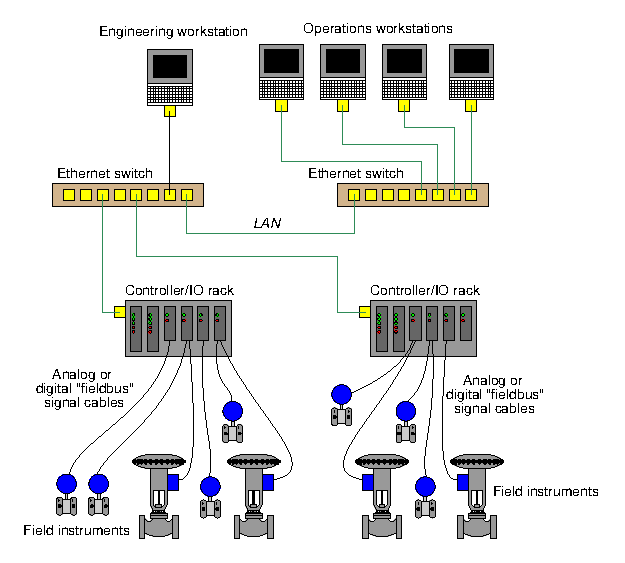
\includegraphics{security_09.eps}$$

It would be wise to configure the PC workstations with password authentication to ensure only authorized personnel have access to the functions of each.  The engineering workstation in particular needs to be protected so that unauthorized personnel do not (either accidently or maliciously) alter critical parameters within the control system essential for proper regulation which could damage the process or otherwise interrupt production.  

\vskip 10pt

\filbreak

\textit{Password timeout} systems introduce a mandatory waiting period for the user if they enter an incorrect password, typically after a couple of attempts so as to allow for innocent entry errors.  \textit{Password lockout} systems completely lock a user out of their digital account if they enter multiple incorrect passwords.  The user's account must then be reset by another user on that system possessing high-level privileges.  \index{Password lockout}  \index{Password timeout}

The concept behind both password timeouts and password lockouts is to greatly increase the amount of time required for any dictionary-style or brute-force password attack to be successful, and therefore deter these attacks.  Unfortunately timeouts and lockouts also present another form of system vulnerability to a \textit{denial of service} attack.  Someone wishing to deny access to a particular system user need only attempt to sign in as that user, using as many incorrect passwords as necessary to trip the automatic lockout.  The timeout or lockout system will then delay (or outright deny) access to the legitimate user.  \index{Denial of service attack}

\vskip 10pt

Authentication based on the user's knowledge (e.g. passwords) is but one form of identification, though.  Other forms of authentication exist which are based on the possession of physical items called \textit{tokens}, as well as identification based on unique features of the user's body (e.g. retinal patterns, fingerprints, facial features) called \textit{biometric} authentication.  

Token-based authentication requires all users to carry tokens on their person.  This form of authentication so long as the token does not become stolen or copied by a malicious party.

Biometric authentication enjoys the advantage of being extremely difficult to replicate and nearly\footnote{Before you laugh at the idea of losing one's own body, consider something as plausible as a fingerprint scanner programmed to accept the image of al fingers on one hand, and then that user suffering an injury to one of the fingers on that hand either obscuring the fingerprint or destroying the finger entirely.} impossible to lose.  The hardware required to scan fingerprints is relatively simple and inexpensive.  Retinal scanners are more complex, but not beyond the reach of organizations possessing expensive digital assets.  Presumably, there will even be DNA-based authentication technology available in the future.






\filbreak
\subsection{Air gaps}

An \textit{air gap} is precisely what the name implies: a physical separation between the critical system network and any other data network preventing communication.  Although it seems so simple that it ought to be obvious, an important design question to ask is whether or not the system in question really needs to have connectivity at all.  Certainly, the more networked the system is, the easier it will be to access useful information and perform useful operational functions.  However, connectivity is also a liability: that same convenience makes it easier for attackers to gain access.  \index{Air gap, network}

Consider the following diagram, showing a simplified example of an industrial control system network (the Control System Local Area Network, or \textit{CS LAN}) ``air gapped'' from the facility's IT network (the \textit{IT LAN}):

$$\includegraphics{security_08.eps}$$

The air gap between the two Ethernet-based networks not only preclude any direct data transfer between one and the other, but also ensure their respective data traffic never collides.  This simple design should be used whenever possible, as it is simple and effective on multiple fronts.

\vskip 10pt

While it may seem as though air gaps are the ultimate solution to digital security because they absolutely prohibit direct network-to-network data transfer, they are not invincible.  A control system that \textit{never} connects to a network other than its own is still vulnerable to cyber-attack via detachable programming and data-storage devices.  For example, one of the controllers in the example control system may become compromised by way of an infected flash data drive plugged into the Engineering Workstation computer. 

\vskip 10pt

\filbreak

In order for air gaps to be completely effective, they must be permanent and include portable devices as well as network connections.  This is where effective security policy comes into play, ensuring portable devices are not allowed into areas where they might connect (intentionally or otherwise) to critical systems.  Effective air-gapping of critical networks also necessitates physical security of the network media: ensuring attackers cannot gain access to the network cables themselves, so as to ``tap'' into those cables and thereby gain access.  This requires careful planning of cable routes and possibly extra infrastructure (e.g. separate cable trays, conduits, and access-controlled equipment rooms) to implement.

\vskip 10pt

Wireless (radio) data networks pose a special problem for the ``air gap'' strategy, because the very purpose of radio communication is to bridge physical air gaps.  A partial measure applicable to some wireless systems is to use \textit{directional antennas} to link separated points together, as opposed to \textit{omnidirectional} antennas which transmit and receive radio energy equally in all directions.  This complicates the task of ``breaking in'' to the data communication channel, although it is not 100 percent effective since no directional antenna has a perfectly focused radiation pattern, nor do directional antennas preclude the possibility of an attacker intercepting communications directly between the two antennae.  Like all security measures, the purpose of using directional antennas is to make an attack \textit{less probable}.








\filbreak
\subsection{Firewalls}

Digital networks should be separated into different \textit{areas} or \textit{layers} in order to reduce their exposure to sources of harm.  A network ``air gap'' is an extreme form of network segregation, but is impractical when some data must be communicated between networks.  

At the opposite end of the network segregation spectrum is a scenario where all digital devices, control systems and office computers alike, connect to the facility's common Local Area Network (LAN).  This is a universally bad policy, as it invites a host of problems not limited to cyber-attacks but extending well beyond that to innocent mistakes and routine faults which may compromise system integrity.  At the very least, control systems deserve their own dedicated network(s) on which to communicate, free of traffic from general information technology (IT) office systems.  The following illustration shows a very poorly-designed network for an industrial facility, where all computers share a common LAN, and are all connected to the internet: \index{LAN, computer}

$$\includegraphics{security_07.eps}$$

In facilities where control system data absolutely must be shared on the general LAN, or shared with an external network such as a WAN or the internet, a \textit{firewall} should be used to connect those two networks.  Firewalls are either software or hardware entities designed to filter data passed through based on pre-set rules.  These rules are stored in a list called an \textit{Access Control List}, or \textit{ACL}.  In essence, each network on either side of a firewall is a ``zone'' of communication, while the firewall is a ``conduit'' between zones allowing only certain types of messages through.  A rudimentary firewall might be configured to ``blacklist'' any data packets carrying hyper-text transfer protocol (HTTP) messages, as a way to prevent web-based access to the system.  Alternatively, a firewall might be configured to ``whitelist'' only data packets carrying Modbus messages for a control system and block everything else.  \index{Firewall, computer}  \index{Access Control List}  \index{ACL, firewall}

Firewalls are standard in IT networks, and have been used successfully for many years.  They may exist as discrete hardware devices with multiple network cable jacks (at minimum one in and one out) screening data traffic between two or more LAN segments, or as software applications running under the operating system of a personal computer to screen data traffic in and out of that PC.

A revised version of the previous industrial network diagram shows how a firewall device could be inserted in such a way as to segregate the LAN into two sub-networks, one for the control system and another for general use:

$$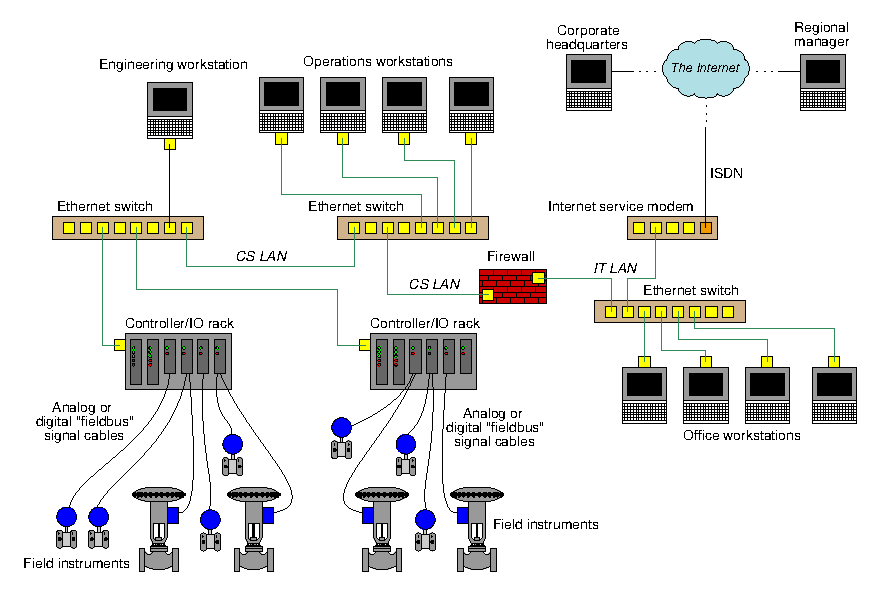
\includegraphics{security_10.eps}$$

With this firewall in place between the CS and IT networks, and configured with appropriate rules governing the passage of data between the two networks, the control system will be more secure from outside eavesdropping or attack than it was before.  For example, data packets received by the firewall from questionable sources on the internet may be denied, while data packets received from known-legitimate sources may be permitted.  Certain destination addresses, such as the IP addresses of the controllers themselves, may be blocked from receiving any data originating on the IT LAN, since only the Operations and Engineering workstations should ever need to send data to the controllers.

Similarly, another firewall could be inserted between the IT LAN's Ethernet switch and the Internet service modem for the purpose of screening data flowing between the IT LAN and the outside world.  This would add a measure of security to the facility's IT network.

\vskip 10pt

\filbreak

Firewall configuration is an area where stark differences may be seen between the control system (CS) versus information technology (IT) worlds.  In the IT world, the job of a firewall is to permit passage of an extremely diverse legitimate data traffic while blocking very specific forms of data.  In the CS world, most legitimate data is of a very limited type and occurs between a very limited number of devices, while all other data is considered illegitimate.  For this reason, it is more common to see IT firewalls employ a ``blacklist'' policy where all data is permitted \textit{except} for types specifically blacklisted in the ACL rules, while CS firewalls commonly employ a ``whitelist'' policy where all data is denied unless specifically permitted in the ACL rules.  \index{Blacklist}  \index{Whitelist}

For example, below you will see a few ``blacklist'' rules taken from a typical \texttt{iptables}\footnote{For the curious, \texttt{iptables} is an administration-level utility application for Linux operating systems, used to edit the ACL rulebase of the operating system's built-in software firewall.  Each line of text in these examples is a command that may be typed manually at the command-line interface of the operating system, or more commonly written to a \textit{script} file to be automatically read and executed upon start-up of the computer.  The \texttt{-A} option instructs \texttt{iptables} to Append a new rule to the ACL.  These rules are organized into groups called ``chains'' which are given names such as \texttt{INPUT} and \texttt{OUTPUT}.  While the specific format of ACL rules are unique to each firewall, they share many common features.} entry for the native firewall within a Linux operating system, intended to reject (``DROP'') any data packets entering the computer from an internet modem connected to Ethernet port 0 (\texttt{eth0}) bearing an IP address within any of the ``private'' ranges\footnote{No device connected directly to the internet should bear an IP address within any of these three ranges, and therefore any data packets received from devices with such an address is immediately suspect.} specified by the Internet Corporation for Assigned Names and Numbers (ICANN):  \index{ICANN}  \index{iptables}

\vskip 10pt

\texttt{iptables -A INPUT -i eth0 -s 10.0.0.0/8 -j DROP}

\texttt{iptables -A INPUT -i eth0 -s 172.16.0.0/12 -j DROP}

\texttt{iptables -A INPUT -i eth0 -s 192.168.0.0/16 -j DROP}

\vskip 10pt

The \texttt{-s} option in \texttt{iptables} specifies a \textit{source} IP address (or range of addresses as shown above), meaning that such a rule is screening data packets based on layer 3 of the OSI Reference model.  Firewalls also provide the means to screen data based on TCP ports which exist at layer 4 of the OSI model, as seen in this next example:  \index{OSI Reference Model}  \index{TCP}

\vskip 10pt

\texttt{iptables -A INPUT -p tcp --dport http -j ACCEPT}

\texttt{iptables -A INPUT -p tcp --dport ssh -j ACCEPT}

\vskip 10pt

Here, the \texttt{-p} option (\textit{protocol}) specifies screening based on TCP port identification, while the \texttt{--dport} (\textit{destination port}) option specifies which TCP port will be identified.  Together, these two rules tell the firewall to permit (``ACCEPT'') all data packets destined for HTTP (web page) or SSH (Secure SHell) ports on external devices, and serve as examples of ``whitelist'' rules in an ACL.  \index{HTTP}  \index{SSH}

\vskip 10pt

\filbreak

Basic firewall behavior is based on screening packets based on IP address (either source or destination), and/or based on TCP port, and as such provide only minimal fortification against attack.  An example of a crude denial of service attack thwarted by a simple firewall rule is a \textit{ping flood}.  Ping is a network diagnostic utility that is part of the ICMP (Internet Control Message Protocol) suite used to test for connection between two IP-aware devices, and it works by having the receiving device reply to the sending device's query.  These queries and replies are very simple and consist of very small amounts of data, but if a device is repeatedly ``pinged'' by one or more machines it may become so busy answering ping requests that it cannot do anything else on the network.  An example of an ACL rule thwarting this crude attack is as follows:  \index{ICMP}  \index{Internet Control Message Protocol}  \index{Echo Request, ICMP} 

\vskip 10pt

\texttt{iptables -A INPUT -p icmp --icmp-type echo-request -j DROP}

\vskip 10pt

With this rule in place, the firewall will deny (``DROP'') all echo-request (i.e. ping) queries.  This, of course, will prevent anyone from every using \texttt{ping} to diagnose a connection to the firewalled computer, but it will also prevent ping flood attacks.

\vskip 10pt

Many modern firewalls offer \textit{stateful inspection} of data packets, referring to the firewall's ability to recognize and log the state of each connection.  TCP, for example, uses a ``handshaking'' procedure involving simple SYN (``synchronize'') and ACK (``acknowledge'') messages sent back and forth between two devices to confirm a reliable connection before any transmitting any data.  A stateful firewall will track the progress of this SYN/ACK ``handshake'' sequence and reject any data from reaching the destination device if they do not agree with the firewall's logged state of that sequence.  Such screening ability filters other types of denial of service attacks which are based on exploitation of this handshake (e.g. a TCP SYN flood attack\footnote{If a TCP-capable device receives too many SYN (``synchronize'') messages in rapid succession, it may lock up and refuse to accept any others.}).  \index{TCP SYN flood attack}

Stateful inspection is only useful, of course, for state-based protocols such as TCP.  UDP is a notably \textit{stateless} protocol that is often used for industrial data because the protocol itself is much simpler than TCP and therefore easier to implement in limited hardware such as within the processor of a PLC.  \index{UDP}

\vskip 10pt

Some specialized firewalls are manufactured specifically for industrial control systems.  One such firewall at the time of this writing (2016) is manufactured by Tofino, and has the capability to screen data packets based on rules specific to industrial control system platforms such as popular PLC models.  Industrial firewalls differ from general-purpose data firewalls in their ability to recognize control-specific data, which exists at layer 7 of the OSI Reference model.  This is popularly referred to as \textit{Deep Packet Inspection}, or \textit{DPI}, because the firewall inspects the contents of each packet (not just source, destination, port, and connection state) for legitimacy.  \index{Tofino industrial network firewall}  \index{OSI Reference Model}  \index{Deep Packet Inspection}  \index{DPI firewall}

Two significant challenges complicate Deep Packet Inspection for any industrial control system.  The first challenge is that the firewall must be fluent in the control system's command structure to be able to discern between legitimate and illegitimate data.  Thus, DPI firewalls must be pre-loaded with files describing what legitimate control system data and data exchange sequences looks like.  Any upgrade of the control system's network involving changes to the protocol necessitates upgrading of the DPI firewall as well.  The second challenge is that the firewall must perform this deep inspection fast enough that the added latency will not compromise control system performance.  The more comprehensive the DPI algorithm, the longer each message will be delayed by the inspection, and the slower the network will be.









\filbreak
\subsection{Demilitarized Zones}

For all its complexity, a network firewall really only provides limited security in limiting data communication between two networks.  This is especially true of stateless firewalls which only screen data based on such criteria as IP addresses and TCP ports.  One way to augment the effectiveness of firewalls is to use multiple firewalls to build something referred to as a \textit{DeMilitarized Zone}, or \textit{DMZ}.  A DMZ consists of three basic elements: a \textit{data server} or \textit{proxy} computer sandwiched between two firewalls.  The purpose of a DMZ is to force all data traffic between the segregated networks to pass through the server/proxy device and prohibit any form of direct network-to-network communication.  Meanwhile, the server/proxy device is programmed with limited functionality to only process legitimate data between the two networks.  \index{DMZ}  \index{Demilitarized Zone}

An example of a DMZ applied to our industrial control system appears in the following diagram.  Please note that the two firewall symbols shown here merely represent firewall \textit{functions} and need not exist as two physical devices.  It is possible to build a DMZ using a single special-purpose device with multiple Ethernet ports and dual firewall ACLs:

$$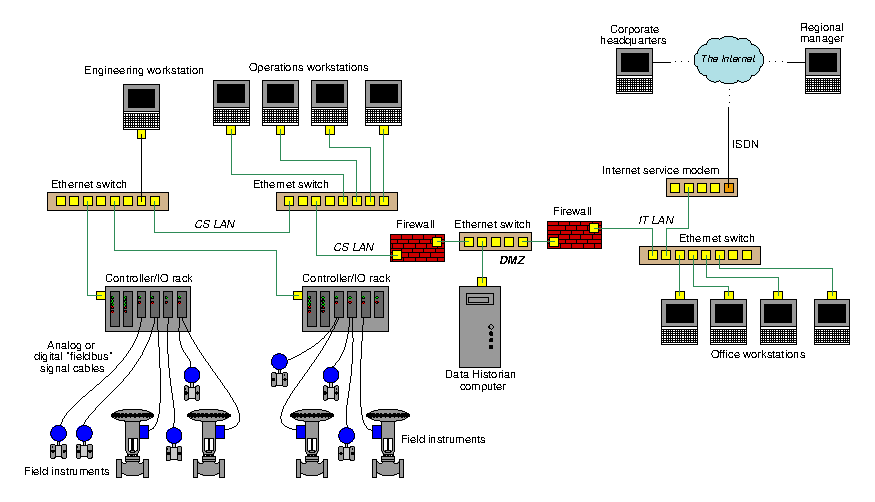
\includegraphics{security_11.eps}$$

\vskip 10pt

\filbreak

For each firewall at the boundary of the DMZ, its respective ACL must be configured so as to only permit (``whitelist'') the Data Historian computer, which is the ``server'' device within the DMZ.  The purpose of a Data Historian is to poll process data from the control system at regular intervals, store that data on a high-capacity data drive, and provide that data (i.e. ``serve the data'') to external computers\footnote{These external computers are called \textit{clients}, and in this network could include the office workstations as well as workstation PCs at corporate headquarters and the regional manager's office.} requesting it.  \index{Data Historian}  \index{Server}  \index{Client}

$$\includegraphics{security_12.eps}$$

Given the fact that it's highly unlikely anyone in a corporate office needs access to real-time process data, the Data Historian's function\footnote{Data Historians have existed in Distributed Control Systems (DCSs) for many years, and in fact pre-date DMZs.  Their purpose during those halcyon days prior to network security concerns was to provide operations and maintenance personnel with long-term data useful for running the process and diagnosing a range of problems.  DCS controllers are typically limited in memory, and simply cannot archive the vast quantities of process data capable within a general-purpose computer.  Their function in modern times as part of an industrial control system DMZ is simply an extension of their original purpose.} will be limited to polling and archiving process data over long periods of time, typically years.  This data, when requested by any user on the IT LAN or beyond, will be provided in convenient form by the Data Historian without need for direct reading from the controllers.  One way to view the function of a server inside of a DMZ is to see it as an \textit{intentional man-in-the-middle} who dispenses information strictly on a need-to-know basis.  \index{Man-in-the-middle}

A DMZ installed in an IT network must convey a much broader range of information, everything from email messages and web pages to large document files and bandwidth-intensive streaming video.  A corporation's \textit{web server}, for example, which is the computer upon which web page files are hosted for view by the outside world, is typically located within a DMZ network.

%% Control system DMZ = servers in the DMZ include data historians, web servers, OPC servers, etc.

Any cyber-attack on a system shielded behind a DMZ must first compromise one or more of the devices lying within the DMZ before any assault may be launched against the protected network, since the dual firewalls prohibit any direct network-to-network communication.  This naturally complicates the task (though, as with any fortification, it can never \textit{prevent} a breach) for the attacker.  The DMZ device's security therefore becomes an additional layer of protection to whatever fortifications exist within the protected LAN.

%% Mention Gateway devices intended to bridge disparate networks???









\filbreak
\subsection{Encryption}

Encryption refers to the intentional scrambling of data by means of a designated code called a \textit{key}, a similar (or in some cases identical) key being used to un-scramble (decrypt) that data on the receiving end.  The purpose of encryption, of course, is to foil passive attacks by making the data unintelligible to anyone but the intended recipient, and also to foil active attacks by making it impossible for an attacker's transmitted message to be successfully received.  \index{Encryption}  \index{Decryption}  \index{Key, cryptographic}

The strength of any encryption method lies in the key used to encrypt and decrypt the protected data, and so these keys should be managed with similar care as passwords.  If the key becomes known to anyone other than the intended users, the encryption becomes worthless.  It is for this reason that many encryption systems provide the feature of \textit{key rotation}, whereby keys are periodically randomized.  Just prior to switching to a new key, the new key's value is communicated with all other devices in the cryptographic system as a piece of encrypted data.  \index{Key rotation}

\vskip 10pt

A popular form of encrypted communication is a \textit{Virtual Private Network} or VPN.  This is where two or more devices use VPN software (or multiple VPN hardware devices) to encrypt messages sent to each other over an unsecure network.  Since the data exchanged between the two computers is encrypted, the communication will be unintelligible to anyone else who might eavesdrop on that unsecure network.  In essence, VPNs create a secure ``tunnel'' for data to travel between points on an otherwise unprotected network.  \index{Virtual Private Network}  \index{VPN}

A popular use for VPN is securing remote access\footnote{Like all tools, VPN must be used with care.  What follows is a cautionary tale.  A controls engineer was hired to do PLC programming at an industrial facility, and the technical staff there insisted he connect his portable computer to the facility's PLC network via a VPN so that he could work via the internet.  This limited his need to be on-site by ensuring he could securely upload, edit, and download code to PLC systems from any location.  After completing the job and traveling to a different client to do more PLC programming work, this engineer accidently logged into the old client's VPN and placed one of their operating PLCs in Stop mode, causing a loss of control on a major process there, \textit{hundreds of miles away from where he was}.  Apart from the lesson of carefully checking login parameters when initiating a VPN connection, this example shows just how vulnerable some industrial control systems are and how over-confident some people are in tools such as VPN to protect their digital assets!  Just because a VPN promises secure communication does not mean it is therefore safe to allow low-level access to control system components along public networks.} to corporate networks, such as when business executives, salespersons, and engineers must do work while away from the facility site.  By ``tunneling'' through to the company network via VPN, all communications between the employee's personal computer and the device(s) on the other end are unintelligible to eavesdroppers.

IP-based networks implement VPN tunneling by using an extension of the IP standard called \textit{IPsec} (IP security), which works by encrypting the original IP packet payload and then encapsulating that encrypted data as the payload of a new (larger) IP packet.  In its strongest form IPsec not only encrypts the original payload but also the original IP header which contains information on IP source and destination addresses.  This means any eavesdropping on the IPsec packet will reveal nothing about the original message, where it came from, or where it's going.  \index{IPsec} 

\vskip 10pt

Encryption may also be applied to non-broadcast networks such as telephone channels and serial data communication lines.  Special cryptographic modems and serial data translators are manufactured specifically for this purpose, and may be applied to legacy SCADA and telemetry networks using on telephony or serial communication cables.

\vskip 10pt

It should be noted that encryption does not necessarily protect against so-called \textit{replay} attacks, where the attacker records a communicated message and later re-transmits that same message to the network.  For example, if a control system uses an encrypted message to command a remotely-located valve to shut, an attacker might simply re-play that same message at any time in the future to force the valve to shut without having to decrypt the message.  So long as the encryption key has not changed between the time of message interception and the time of message re-play, the re-played message should be interpreted by the receiving device the same as before, to the same effect.  Key rotation therefore becomes an important element in fortifying simplex messages against replay attacks, because a new key will necessarily alter the message from what it was before and thereby render the old (intercepted) message meaningless.

\vskip 10pt

An interesting form of encryption applicable to certain wireless (radio) data networks is \textit{spread-spectrum} communication.  This is where radio communication occurs over a range of different frequencies rather than on a single frequency.  Various techniques exist for spreading digital data across a spectrum of radio frequencies, but they all comprise a form of data encryption because the spreading of that data is orchestrated by means of a cryptographic key.  Perhaps the simplest spread-spectrum method to understand is \textit{frequency-hopping} or \textit{channel-hopping}, where the transmitters and receivers both switch frequencies on a keyed schedule.  Any receiver uninformed by the same key will not ``know'' which channels will be used, or in what order, and therefore will be unable to intercept anything but isolated pieces of the communicated data.  Spread-spectrum technology was invented during the second World War as a means for Allied forces to encrypt their radio transmissions such that Axis forces could not interpret them.  \index{Spread-spectrum radio}

Spread-spectrum capability is built into several wireless data communication standards, including Bluetooth and \textsl{Wireless}HART.  \index{WirelessHART}  \index{Bluetooth}

\vskip 10pt

Network communication is not the only form of data subject to encryption.  Static files stored on computer drives may also be encrypted, such that only users possessing the proper key(s) may decrypt and use the files.  This fortification is especially useful for securing data stored on portable media such as flash memory drives, which may easily fall into malevolent hands.

%ADD: footnote on Hedy Lamarr's role in the invention of spread-spectrum radio








\filbreak
\subsection{Read-only system access}

One way to thwart so-called ``active'' attacks (where the attacker inserts or modifies data in a digital system to achieve malicious ends) is to engineer the system in such a way that all communicated data is \textit{read-only} and therefore cannot be written or edited by anyone.  This, of course, by itself will do nothing to guard against ``passive'' (read-only) attacks such as eavesdropping, but passive attacks are definitely the lesser of the two evils with regard to industrial control systems.

In systems where the digital data is communicated serially using protocols such as EIA/TIA-232, read-only access may be ensured by simply disconnecting one of the wires in the EIA/TIA-232 cable.  By disconnecting the wire leading to the ``receive data'' pin of the critical system's EIA/TIA-232 serial port, that system cannot receive external data but may only transmit data.  The same is true for EIA/TIA-485 serial communications where ``transmit'' and ``receive'' connection pairs are separate.  \index{EIA/TIA-232 serial communication}  \index{RS-232 serial communication}  \index{EIA/TIA-485 serial communication}  \index{RS-485 serial communication}

Certain serial communication schemes are inherently simplex (i.e. one-way communication) such as EIA/TIA-422.  If this is an option supported by the digital system in question, the use of that option will be an easy way to ensure remote read-only access.  \index{EIA/TIA-422 serial communication}  \index{RS-422 serial communication}

\vskip 10pt

For communication standards such as Ethernet which are inherently duplex (bi-directional), devices called \textit{data diodes} may be installed to ensure read-only access.  The term ``data diode'' invokes the functionality of a semiconductor rectifying diode, which allows the passage of electric current in one direction only.  Instead of blocking reverse current flow, however, a ``data diode'' blocks reverse \textit{information} flow.  \index{Ethernet}  \index{Data diode}

\vskip 10pt

The principle of read-only protection applies to computing systems as well as communication networks.  Some digital systems do not strictly require on-board data collection or modification of operating parameters, and in such cases it is possible to replace read/write magnetic data drives with read-only (e.g. optical disk) drives in order to create a system that cannot be compromised.  Admittedly, applications of this strategy are limited, as there are few control systems which never store operational data nor require any editing of parameters.  However, this strategy should be considered where it applies\footnote{An example of this strategy in action is an internet-connected personal computer system I once commissioned, running the Linux operating system from a DVD-ROM optical disk rather than a magnetic hard drive.  The system would access the optical disk upon start-up to load the operating system kernel into its RAM memory, and then access the disk as needed for application executable files, shared library files, and other data.  The principal use of this system was web browsing, and my intent was to make the computer as ``hacker-proof'' as I possibly could.  Since the operating system files were stored on a read-only optical disk, it was impossible for an attacker to modify that data without having physical access to the machine.  In order to thwart attacks on the data stored in the machine's RAM memory, I configured the system to automatically shut down and re-start every day at an hour when no one would be using it.  Every time the computer re-booted, its memory would be a \textit{tabula rasa} (``clean slate'').  Of course, this meant no one could permanently store downloaded files or other data on this machine from the internet, but from a security perspective that was the very point.}.

\vskip 10pt

Many digital devices offer \textit{write-protection} features in the form of a physical switch or key-lock preventing data editing.  Just as some types of removable data drives have a ``write-protect'' tab or switch located on them, some ``smart'' field instruments also have write-protect switches inside their enclosures which may be toggled only by personnel with direct physical access to the device.  Programmable Logic Controllers (PLCs) often have a front-panel write-protect switch allowing protection of the running program.  

Not only do write-protect switches guard against malicious attacks, but they also help prevent innocent mistakes from causing major problems in control systems.  Consider the example of a PLC network where each PLC connected to a common data network has its own hardware write-protect switch.  If a technician or engineer desires to edit the program in one of these PLCs from their remotely-located personal computer, that person must first go to the location of that PLC and disable its write protection.  While this may be seen as an inconvenience, it ensures that the PLC programmer will not mistakenly access the wrong PLC from their office-located personal computer, which is especially easy to do if the PLCs are similarly labeled on the network.

Making regular use of such features is a policy measure, but ensuring the exclusive use of equipment with this feature is a system design measure.







\filbreak
\subsection{Control platform diversity}

In control and safety systems utilizing redundant controller platforms, an additional measure of security is to use different models of controller in the redundant array.  For example, a redundant control or safety system using two-out-of-three voting (2oo3) between three controllers might use controllers manufactured by three different vendors, each of those controllers running different operating systems and programmed using different editing software.  This mitigates against device-specific attacks, since no two controllers in the array should have the exact same vulnerabilities.  

A less-robust approach to process control security through diverse platforms is simply the use of effective Safety Instrumented Systems (SIS) applied to critical processes, which always employ controls different from the base-layer control system.  An SIS system is designed to bring the process to a safe (shut down) condition in the event that the regular control system is unable to maintain normal operating conditions.  In order to avoid common-cause failures, the SIS must be implemented on a control platform independent from the regular control system.  The SIS might even employ analog control technology (and/or discrete relay-based control technology) in order to give it complete immunity from digital attacks.

In either case, improving security through the use of multiple, diverse control systems is another example of the \textit{defense in depth} philosophy in action: building the system in such a way that no essential function depends on a single layer or single element, but rather multiple layers exist to ensure that essential function.

%A similar strategy would be to use non-networked (or even non-digital) controllers within the redundant array.  
















%\filbreak
%\subsection{Cryptographic techniques}






%\filbreak
%\subsubsection{Cryptographic keys}

%ADD: symmetric key encryption (private keys)
%     --> Simple and fast
%     --> Problem: how to securely distribute the private key?

%ADD: asymmetric key encryption (public/private keys)
%     --> Public key (anyone can have) is only good for encryption, not decryption
%     --> Private key (only the receiver has) is used for decryption
%     --> Complex and slow
%     --> Key distribution problem solved!

%ADD: hybrid systems (use asymmetric key encryption to distribute private keys to all parties)



%\filbreak
%\subsubsection{Cryptographic algorithms}

%ADD: Caesar Cipher (shifting letters in the alphabet by a fixed offset)
%     --> Refer to Ted Fischer's "Ransomware" tutorial for more details
%     --> The offset value is the private key
%ADD: XOR encryption/decryption
%     --> The XOR'd value is the private key







\filbreak
\section{Policy-based fortifications}

These fortifications focus on human behavior rather than system design or component selection.  In some ways these are the simplest to implement, as they generally require little in the way of technical expertise.  This is not to suggest, however, that policy-based fortifications are therefore the \textit{easiest} to implement.  On the contrary, changing human behavior is usually a very difficult feat.  Policy-based fortifications are not necessarily cheap, either: although little capital is generally required, operational costs will likely rise as a result of these policies.  This may take the form of monetary costs, additional staffing costs, and/or simply costs associated with impeding normal work flow (e.g. pulling personnel away from their routine tasks to do training, requiring personnel to spend more time doing things like inventing and tracking new passwords, slowing the pace of work by limiting authorization).






\filbreak
\subsection{Foster awareness}

Ensure all personnel tasked with using and maintaining the system are fully aware of security threats, and of best practices to mitigate those threats.  Given the ever-evolving nature of cyber-attacks, this process of educating personnel must be continuous.

A prime mechanism of cyber-vulnerability is the casual sharing of information between employees, and with people outside the organization.  Information such as passwords and network design should be considered ``privileged'' and should only be shared on a need-to-know basis.  Critical security information such as passwords should never be communicated to others or stored electronically in plain (``cleartext'') format.  When necessary to communicate or store such information electronically, it should be encrypted so that only authorized personnel may access it.

In addition to the ongoing education of technical personnel, it is important to keep management personnel aware of cyber threat and threat potentials, so that the necessary resources will be granted toward cyber-security efforts. 

%ADD: all personnel using the system must adhere to sensible security guidelines
%ADD: training (what to do) and education (why)






\filbreak
\subsection{Employ security personnel}

For any organization managing important processes and services, ``important'' being defined here as \textit{threatening} if compromised by the right type of cyber-attack, it is imperative to employ qualified and diligent personnel tasked with the ongoing maintenance of digital security.  These personnel must be capable of securing the control systems themselves and not just general data systems.

One of the routine tasks for these personnel should be evaluations of risks and vulnerabilities.  This may take the form of security audits or even simulated attacks whereby the security of the system is tested with available tools.






\filbreak
\subsection{Utilize effective authentication}

Simply put, it is imperative to correctly identify all users accessing a system.  This is what ``authentication'' means: correctly identifying the person (or device) attempting to use the digital system.  \textit{Passwords} are perhaps the most common authentication technique.  \index{Passwords}

\vskip 10pt

The first and foremost precaution to take with regard to authentication is to never use default (manufacturer) passwords, since these are public information.  This precautionary measure may seem so obvious as to not require any elaboration, but sadly it remains a fact that too many password-protected devices and systems are found operating in industry with default passwords.

Another important precaution to take with passwords is to not use the same password for all systems.  The reasoning behind this precaution is rather obvious: once a malicious party gains knowledge of that one password, they have access to all systems protected by it.  The scenario is analogous to using the exact same key to unlock every door in the facility: all it takes now is one copied key and suddenly intruders have access to every room.

Passwords must also be changed on a regular basis.  This provides some measure of protection even after a password becomes compromised, because the old password(s) no longer function.

\vskip 10pt

Passwords chosen by system users should be ``strong,'' meaning difficult for anyone else to guess.  When attackers attempt to guess passwords, they do so in two different ways:

\begin{itemize}
\item Try using common words or phrases that are easy to memorize
\item Try every possible combination of characters until one is found that works
\end{itemize}

The first style of password attack is called a \textit{dictionary attack}, because it relies on a database of common words and phrases.  The second style of password attack is called a \textit{brute force attack} because it relies on a simple and tireless (``brute'') algorithm, practical only if executed by a computer.  \index{Dictionary attack, password}  \index{Brute force attack, password}

A password resistant to dictionary-style attacks is one not based on a common word or phrase.  Ideally, that password will appear to be nonsense, not resembling any discernible word or simple pattern.  The only way to ``crack'' such a password, since a database of common words will be useless against it, will be to attempt every possible character combination (i.e. a brute-force attack).

A password resistant to brute-force-style attacks is one belonging to a huge set of possible passwords.  In other words, there must be a very large number of possible passwords limited to the same alphabet and number of characters.  Calculating the brute-force strength of a password is a matter of applying a simple exponential function:

$$S = C^n$$

\noindent
Where,

$S$ = Password strength (i.e. the number of unique password combinations possible)

$C$ = Number of available characters (i.e. the size of the alphabet)

$n$ = Number of characters in the password

\vskip 10pt

\filbreak

For example, a password consisting of four characters, each character being a letter of the English alphabet where lower- and upper-case characters are treated identically, would give the following strength:

$$S = 26^4 = 456976 \hbox{ possible password combinations}$$

If we allowed case-sensitivity (i.e. lower- and upper-case letters treated differently), this would double the value of $C$ and yield more possible passwords: 

$$S = 52^4 = 7311616 \hbox{ possible password combinations}$$

%ADD: expand "C" by adding numbers and then symbols

Obviously, then, passwords using larger alphabets are stronger than passwords with smaller alphabets.

%ADD: however, the REAL gains in password strength come from longer passwords (greater "n"), for the simple reason that exponential functions grow faster than power functions.


%ADD: strong, private passwords
%ADD: measuring password strength:
%     --> Relative: avoiding common words (protects against "dictionary" attacks)
%     --> Absolute: maximize N (protects against "dictionary" and "brute force" attacks)
%         --> 62-cipher alphabet, 10 characters long = 8.393e17 combinations
%         --> 62-cipher alphabet, 11 characters long = 5.204e19 combinations
%         --> 62-cipher alphabet, 12 characters long = 3.226e21 combinations
%         --> 62-cipher alphabet, 13 characters long = 2.000e23 combinations
%         --> 62-cipher alphabet, 15 characters long = 7.689e26 combinations
%         --> 62-cipher alphabet, 20 characters long = 7.044e35 combinations
%         --> 62-cipher alphabet, 25 characters long = 6.453e44 combinations

%         --> 52-cipher alphabet, 10 characters long = 1.446e17 combinations
%         --> 62-cipher alphabet, 10 characters long = 8.393e17 combinations
%         --> 72-cipher alphabet, 10 characters long = 3.744e18 combinations
%         --> 82-cipher alphabet, 10 characters long = 1.374e19 combinations

%         --> 52-cipher alphabet, 15 characters long = 5.496e25 combinations
%         --> 62-cipher alphabet, 15 characters long = 7.689e26 combinations
%         --> 72-cipher alphabet, 15 characters long = 7.244e27 combinations
%         --> 82-cipher alphabet, 15 characters long = 5.096e28 combinations

%         --> 52-cipher alphabet, 20 characters long = 2.090e34 combinations
%         --> 62-cipher alphabet, 20 characters long = 7.044e35 combinations
%         --> 72-cipher alphabet, 20 characters long = 1.402e37 combinations
%         --> 82-cipher alphabet, 20 characters long = 1.889e38 combinations

%         --> 2-cipher alphabet, 128 characters long = 3.403e38 combinations
%
%     --> Lesson: password length matters more than password alphabet size!

%ADD: never use factory-default passwords!
%ADD: how to archive passwords safely
%     --> Don't do it in any digital form open to networking!
%ADD: lockouts with incorrect password entries
%ADD: password rotation (foils existing compromises)
%ADD: token-based authentication (RFID scan cards, USB dongles)
%ADD: biometric authentication (retinal scans, fingerprint scans, DNA scans)







\filbreak
\subsection{Cautiously grant authorization}

While \textit{authentication} is the process of correctly identifying the user, \textit{authorization} is the process of assigning rights to each user.  The two concepts are obviously related, but not identical.  Under any robust security policy, users are given only as much access as they need to perform their jobs efficiently.  Too much access not only increases the probability of an attacker being able to cause maximum harm, but also increases the probability that benevolent users may accidently cause harm.

Perhaps the most basic implementation of this policy is for users to log in to their respective computers using the lowest-privilege account needed for the known task(s), rather than to log in at the highest level of privilege they \textit{might} need.  This is a good policy for all people to adopt when they use personal computers to do any sort of task, be it work- or leisure-related.  Logging in with full (``administrator'') privileges is certainly convenient because it allows you to do anything on the system (e.g. install new software, reconfigure any service, etc.) but it also means any malware accidently engaged\footnote{Consider the very realistic scenario of logging in as administrator (or ``root'' in Unix systems) and then opening an email message which happens to carry an attached file infected with malware.  Any file executed by a user is by default run at that user's level of privilege because the operating system assumes that is the user's intent.} under that account now has the same unrestricted level of access to the system.  Habitually logging in to a computer system with a low-privilege account helps mitigate this risk, for any accidental execution of malware will be similarly limited in its power to do harm.  \index{Administrator privilege, computer}  \index{Root privilege, computer}

Another implementation of this policy is called \textit{application whitelisting}, where only trusted software applications are allowed to be executed on any computer system.  This stands in contrast to ``blacklisting'' which is the philosophy behind anti-virus software: maintaining a list of software applications known to be harmful (malware) and prohibiting the execution of those pre-identified applications.   Blacklisting (anti-virus) only protects against malware that has been identified and notified to that computer.  Blacklisting cannot protect against ``zero-day'' malware known by no one except the attacker.  In a whitelisting system, each computer is pre-loaded with a list of acceptable applications, and no other applications -- benign or malicious -- will be able to run on that machine.   \index{Blacklisting, application}  \index{Whitelisting, application}  \index{Application whitelisting, computer}  \index{Application blacklisting, computer}  \index{Anti-virus, computer}

%ADD: default to "no access", then grant access to specific users as necessary







\filbreak
\subsection{Maintain good documentation}

While this is important for effective maintenance in general, thorough and accurate documentation is especially important for digital security because it helps identify vulnerabilities.  Details to document include:

\begin{itemize}
\item Network diagrams
\item Software version numbers
\item Device addresses
\end{itemize}







\filbreak
\subsection{Close unnecessary access pathways}

All access points to the critical system must be limited to those necessary for system function.  This means all other potential access points in the critical system must be closed so as to minimize the total number of access points available to attackers.  Examples of access points which should be inventoried and minimized:

\begin{itemize}
\item Hardware communication ports (e.g. USB serial ports, Ethernet ports, wireless radio cards)
\item Software TCP ports
\item Shared network file storage (``network drives'')
\item ``Back-door'' accounts used for system development
\end{itemize}

\index{Ethernet}

That last category deserves some further explanation.  When engineers are working to develop a new system, otherwise ordinary and sensible authentication/authorizations measures become a major nuisance.  The process of software development always requires repeated logins, shutdowns, and tests forcing the user to re-authenticate themselves and negotiate security controls.  It is therefore understandable when engineers create simpler, easier access routes to the system under development, to expedite their work and minimize frustration.  

Such ``back-door'' access points become a problem when those same engineers forget (or simply neglect) to remove them after the developed system is released for others to use.  An interesting example of this very point was the so-called \textit{basisk} vulnerability discovered in some Siemens S7 PLC products.  A security researcher named Dillon Beresford working for NSS Labs discovered a telnet\footnote{Telnet is a legacy software utility used to remotely access command-line computer operating systems.  Inherently unsecure, telnet exchanges login credentials (user name and password) unencrypted over the network connection.  A modern replacement for telnet is SSH (Secure SHell).} service running on certain models of Siemens S7 PLCs with a user account named ``basisk'' (the password for this account being the same as the user name).  All one needed to do in order to gain privileged access to the PLC's operating system was connect to the PLC using a telnet client and enter ``basisk'' for the user name and ``basisk'' for the password!  Clearly, this was a back-door account used by Siemens engineers during development of that PLC product line, but it was not closed prior to releasing the PLC for general use.  \index{Beresford, Dillon}  \index{NSS Labs}  \index{Siemens S7-300 PLC}  \index{basisk Siemens PLC exploit}  \index{TELNET}  \index{SSH}   \index{Passwords} 








\filbreak
\subsection{Maintain operating system software}

All operating system software manufacturers periodically release ``patches'' designed to improve the performance of their products.  This includes patches for discovered security flaws.  Therefore, it is essential for all computers belonging to a critical system to be regularly ``patched'' to ensure maximum resistance to attack.

\vskip 10pt

This is a significant problem within industry because so much industrial control system software is built to run on consumer-grade operating systems such as Microsoft Windows.  Popular operating systems are built with maximum convenience in mind, not maximum security or even maximum reliability.  New features added to an operating system for the purpose of convenient access and/or new functionality often present new vulnerabilities\footnote{I am reminded of an example from the world of ``smart'' mobile telephones, commonly equipped with \textit{accelerometer} sensors for detecting physical orientation.  Accelerometers detect the force of acceleration and of gravity, and are useful for a variety of convenient ``apps'' having nothing to do with telephony.  Smart phone manufacturers include such sensors in their mobile devices and link those sensors to the phone's operating system because doing so permits innovative applications, which in turn makes the product more desirable to application developers and ultimately consumers.  It was discovered, though, that the signals generated by these accelerometers could be used to detect ``keystrokes'' made by the user, the sensors picking up vibrations made as the user taps their finger against the glass touch-screen of the smart phone.  With the right signal processing, the accelerometers' signals could be combined in such a way to identify which characters the user was tapping on the virtual keyboard, and thereby eavesdrop on their text-based communications!}.  \index{Accelerometer}

Another facet to the consumer-grade operating system problem is that these operating systems have relatively short lifespans.  Driven by consumer demand for more features, software manufacturers develop new operating systems and abandon older products at a much faster rate than industrial users upgrade their control systems.  Upgrading the operating systems on computers used for an industrial control system is no small feat, because it usually means disruption of that system's function, not only in terms of the time required to install the new software but also (potentially) re-training required for employees.  Upgrading may even be impossible in cases where the new operating system no longer supports features necessary for that control system\footnote{An example of this is where a piece of obsolete industrial software runs on the computer's operating system, for example a data acquisition program or data-analysis program made by a company that no longer exists.  If this specialized software was written to run on a particular operating system, and no others, future versions of that operating system might not permit proper function of that specialized software.  I have seen such cases in industry, where industrial facilities continue to run obsolete (unsupported) operating systems in order to keep running some specialized industrial software (e.g. PLC programming editors), which is needed to operate or maintain some specialized piece of control hardware which itself is obsolete but still functions adequately for the task.  In order to upgrade to a modern operating system on that computer (e.g. an obsolete version of Microsoft Windows), one must upgrade the specialized software (e.g. the PLC programming editor software), which in turn would mean upgrading the control hardware (e.g. the PLCs themselves).  All of this requires time and money, much more than just what is required to upgrade the operating system software itself.}.  This would not be a problem if operating system manufacturers provided the same long-term (multi-decade) support for their products as industrial hardware manufacturers typically do, but this is not the case for consumer-grade products such as Microsoft Windows\footnote{As a case in point, there are still a great many industrial computers running Microsoft Windows XP at the time of this writing (2016), even though this operating system is no longer supported by Microsoft.  This means no more Service Pack upgrades from Microsoft, security patches, or even research on vulnerabilities for this obsolete operating system.  All users of Windows XP are ``on their own'' with regard to cyber-attacks.}.






\filbreak
\subsection{Routinely archive critical data}

The data input into and generated by digital control systems is a valuable commodity, and must be treated as such.  Unlike material commodities, data is easily replicated, and this fact provides some measure of protection against loss from a cyber-attack.  Routine ``back-ups'' of critical data, therefore, is an essential part of any cyber-security program.  It should be noted that this includes not just operational data collected by the control system during operation, but also data such as:

\begin{itemize}
\item PID tuning parameters
\item Control algorithms (e.g. function block programs, configuration data, etc.)
\item Network configuration parameters
\item Software installation files
\item Software license (authorization) files
\item Software drivers
\item Firmware files
\item User authentication files
\item All system documentation (e.g. network cable diagrams, loop diagrams)
\end{itemize}

This archived data should be stored in a medium immune to cyber-attacks, such as read-only optical disks.  It would be foolish, for example, to store this sort of critical data only as files on the operating drives of computers susceptible to attack along with the rest of the control system.










\filbreak
\subsection{Create response plans}

Just as no industrial facility would be safe without incident response plans to mitigate physical crises, no industrial facility using digital control systems is secure without response plans for cyber-attacks.  This includes such details as:

\begin{itemize}
\item A chain of command for leading the response
\item Instructions on how to restore critical data and system functions
\item Work-arounds for minimal operation while critical systems are still unavailable
\end{itemize}







\filbreak
\subsection{Limit mobile device access}

Mobile digital devices such as cell phones and even portable storage media (e.g. USB ``flash'' drives) pose digital security risks because they may be exploited as an attack vector bypassing air gaps and firewalls.  It should be noted that version 0.5 of Stuxnet was likely inserted into the Iranian control system in this manner, through an infected USB flash drive.

A robust digital security policy will limit or entirely prohibit personal electronic devices into areas where they might connect to the facility's networks or equipment.  Where mobile devices are essential for job functions, those devices should be owned by the organization and registered in such a way as to authenticate their use.  Computers should be configured to automatically reject non-registered devices such as removable flash-memory storage drives.  Portable computers not owned and controlled by the organization should be completely off-limits\footnote{This raises a potential problem from the perspective of outside technical support, since such support often entails contracted or manufacturer-employed personnel entering the site and using their work computers to perform system configuration tasks.  For any organization implementing a strong security access policy, this point will need to be negotiated into every service contract to ensure all the necessary pieces of hardware and software exist ``in-house'' for the service personnel to use while on the job.} from the process control system.

\vskip 10pt

Above all, one should never underestimate the potential harm allowing uncontrolled devices to connect to critical, trusted portions of an industrial control system.  The degree to which any portion of a digital system may be considered ``trusted'' is a function of \textit{every} component of that system.  Allowing connection to untrusted devices violates the confidence of that system.








\filbreak
\subsection{Secure all toolkits}

A special security consideration for industrial control systems is the existence of software designed to create and edit controller algorithms and configurations.  The type of software used to write and edit Ladder Diagram (LD) code inside of programmable logic controllers (PLCs) is a good example of this, such as the Step7 software used to program Siemens PLCs in Iran's Natanz uranium enrichment facility.  Instrumentation professionals use such software on a regular basis to do their work, and as such it is an essential tool of the trade.  However, this very same software is a weapon in the hands of an attacker, or when hijacked by malicious code.

A common practice in industry is to leave computers equipped with such ``toolkit'' software connected to the control network for convenience.  This is a poor policy, and one that is easily remedied by simply disconnecting the programming computer from the control network immediately after downloading the edited control code.  An even more secure policy is to never connect such ``toolkit'' computers to a network at all, but only to controllers directly, so that the toolkit software cannot be hijacked.

Another layer of defense is to utilize robust password protection on the programmable control devices when available, rather than leaving password fields blank which then permits any user of the toolkit software full access to the controller's programming.  \index{Passwords}









\filbreak
\subsection{Close abandoned accounts}

Given the fact that disgruntled technical employees constitute a significant security threat to organizations, it stands to reason that the user accounts of terminated employees should be closed as quickly as possible.  Not only do terminated employees possess authentication knowledge in the form of user names and passwords, but they may also possess extensive knowledge of system design and vulnerabilities.













\filbreak
\section{Review of fundamental principles}

Shown here is a partial listing of principles applied in the subject matter of this chapter, given for the purpose of expanding the reader's view of this chapter's concepts and of their general inter-relationships with concepts elsewhere in the book.  Your abilities as a problem-solver and as a life-long learner will be greatly enhanced by mastering the applications of these principles to a wide variety of topics, the more varied the better.

\begin{itemize}
\item \textbf{Blacklisting}: the concept of flagging certain users, software applications, etc. as ``forbidden' from accessing a system.
\item \textbf{Chemical isotopes}: variants of chemical elements differing fundamentally in atomic mass.  Relevant to the subject of uranium enrichment for nuclear reactors and nuclear weapons, where one particular isotope must be separated from (``enriched'') another isotope in order to be useful.
\item \textbf{Defense-in-Depth}: a design philosophy relying on multiple layers of protection, the goal being to maintain some degree of protection in the event of one or more other layers failing.
\item \textbf{Reliability}: a statistical measure of the probability that a system will perform its design function.  Relevant here with regard to control systems, in that proper control system design can significantly enhance the reliability of a large system if the controls are able to isolate faulted redundant elements within that system.  This is the strategy used by designers of the Iranian uranium enrichment facility, using PLC controls to monitor the health of many gas centrifuges used to enrich uranium, and taking failed centrifuges off-line while maintaining continuous production.
\item \textbf{Whitelisting}: the concept of only permitting certain users, software applications, etc. to access a system.
\end{itemize}


















\filbreak
\section*{References}

% In alphabetical order!
% \noindent
% Lastname, Firstname MiddleI., \textit{Book Title}, Publisher, City, State, Year.
% \vskip 10pt
% \noindent
% Lastname, Firstname MiddleI., \textit{Book Title}, Publisher, City, State, Year.
% etc . . .

\noindent
``21 Steps to Improve Cyber Security of SCADA Networks'', Department of Energy, USA, May 2011.

\vskip 10pt

\noindent
Bartman, Tom and Carson, Kevin, ``Securing Communications for SCADA and Critical Industrial Systems'', Technical Paper 6678-01, Schweitzer Engineering Laboratories, Inc., Pullman, WA, January 22, 2015.

\vskip 10pt

\noindent
Beresford, Dillon, ``Siemens Simatic S7 PLC Exploitation'', technical presentation at Black Hat USA conference, 2011.

\vskip 10pt

\noindent
Byres, Eric, ``Building Intrinsically Secure Control and Safety Systems -- Using ANSI/ISA-99 Security Standards for Improved Security and Reliability'', Byres Security Inc., May 2009.

\vskip 10pt

\noindent
Byres, Eric, ``Understanding Deep Packet Inspection (DPI) for SCADA Security'', document WP\_INDS\_TOF\_514\_A\_AG, Belden, Inc., 2014.

\vskip 10pt

\noindent
Ciampa, Mark, \textit{Security+ Guide to Network Security Fundamentals}, Course Technology (a division of Thompson Learning), Boston, MA, 2005.

\vskip 10pt

\noindent
``Common Cybersecurity Vulnerabilities in Industrial Control Systems'', Department of Homeland Security, Control Systems Security Program, National Cyber Security Division, USA, May 2011.

\vskip 10pt

\noindent
Falliere, Nicolas; Murchu, Liam O.; Chien, Eric; ``W32.Stuxnet Dossier'', version 1.4, Symantec Corporation, Mountain View, CA, February 11, 2011.

\vskip 10pt

\noindent
Fischer, Ted, ``Private and Public Key Cryptography and Ransomware'', Center for Internet Security, Inc., Pullman, WA, December 2014.

\vskip 10pt

\noindent
Grennan, Mark, ``Firewall and Proxy Server HOWTO'', version 0.8, February 26, 2000.

\vskip 10pt

\noindent
Horak, Ray, \textit{Webster's New World Telecom Dictionary}, Wiley Publishing, Inc., Indianapolis, IN, 2008.

\vskip 10pt

\noindent
Kemp, R. Scott, ``Gas Centrifuge Theory and Development: A Review of US Programs'', Program on Science and Global Security, Princeton University, Princeton, NJ, Taylor \& Francis Group, LLC, 2009.

\vskip 10pt

\noindent
Langner, Ralph, ``To Kill A Centrifuge -- A Technical Analysis of What Stuxnet's Creators Tried to Achieve'', The Langner Group, Arlington, MA, November 2013.

\vskip 10pt

\noindent
Lee, Jin-Shyan; Su, Yu-Wei; Shen, Chung-Chou, ``A Comparative Study of Wireless Protocols: Bluetooth, UWB, ZigBee, and Wi-Fi'', Industrial Technology Research Institute, Hsinchu, Taiwan, November 2007.

\vskip 10pt

\noindent
Leidigh, Christopher, ``Fundamental Principles of Network Security'', White Paper \#101, American Power Conversion (APC), 2005.

\vskip 10pt

\noindent
Leischner, Garrett and Whitehead, David, ``A View Through the Hacker's Looking Glass'', Technical Paper 6237-01, Schweitzer Engineering Laboratories, Inc., Pullman, WA, April 2006.

\vskip 10pt

\noindent
Makhijani, Arjun Ph.D.; Chalmers, Lois; Smith, Brice Ph.D.; ``Uranium Enrichment -- Just Plain Facts to Fuel an Informed Debate on Nuclear Proliferation and Nuclear Power'', Institute for Energy and Environmental Research, October 15, 2004.

\vskip 10pt

\noindent
McDonald, Geoff; Murchu, Liam O.; Doherty, Stephen; Chien, Eric; ``Stuxnet 0.5: The Missing Link'', version 1.0, Symantec Corporation, Mountain View, CA, February 26, 2013.

\vskip 10pt

\noindent
Oman, Paul W.; Risley, Allen D.; Roberts, Jeff; Schweitzer, Edmund O. III, ``Attack and Defend Tools for Remotely Accessible Control and Protection Equipment in Electric Power Systems'', Schweitzer Engineering Laboratories, Inc., Pullman, WA, March 12, 2002.

\vskip 10pt

\noindent
Postel, John, \textit{Internet Protocol -- DARPA Internet Program Protocol Specification}, RFC 791, Information Sciences Institute, University of Southern California, Marina Del Ray, CA, September 1981.

\vskip 10pt

\noindent
Rescorla, E. and Korver, B.; ``Guidelines for Writing RFC Text on Security Considerations'' (RFC 3552), The Internet Society, July 2003.

\vskip 10pt

\noindent
Risley, Allen; Marlow, Chad; Oman, Paul; Dolezilek, Dave, ``Securing SEL Ethernet Products With VPN Technology'', Application Guide 2002-05, Schweitzer Engineering Laboratories, Inc., Pullman, WA, July 11, 2002.

\vskip 10pt

\noindent
``Seven Strategies to Effectively Defend Industrial Control Systems'', National Cybersecurity and Communications Integration Center (NCCIC), Department of Homeland Security (DHS), USA.

\vskip 10pt

\noindent
``Tofino Xenon Security Appliance'' data sheet, document DS-TSA-XENON version 6.0, Tofino Security, 2014.

\vskip 10pt

\noindent
``W32.DuQu -- The Precursor to the next Stuxnet'', version 1.4, Symantec Corporation, Mountain View, CA, November 23, 2011.

\vskip 10pt

\noindent
Whitehead, David and Smith, Rhett, ``Cryptography: A Tutorial for Power Engineers'', Technical Paper 6345-01, Schweitzer Engineering Laboratories, Inc., Pullman, WA, October 20, 2008.

\vskip 10pt

\noindent
Zippe, Gernot, ``A Progress Report: Development of Short Bowl Centrifuges'', Department of Physics, University of Virginia, July 1, 1959.

\vskip 10pt

%ADD: APC "Fundamental Principles of Network Security"

















%%%%%%%%%%%%%%%%%%%%%%%%%%%%%%%%%%%%%%%%%%%%%%%%%%%%

